\documentclass[twoside]{projektInzynierskiMS}
\usepackage{polski}
\usepackage[utf8]{inputenc}
\usepackage{amsmath}
\usepackage{graphicx}
%\drukJednostronny

%% tytuł promotor iautor (\title to komenda standardowa)
\title{System obsługi Biblioteki Wydziału Matematyki Stosowanej}
\promotor{dr inż. Marek Xsiński}


%% każdy autor musi mieć 4 argumenty: imię nazwisko, nr albumu, procent wkładu, opis wkładu
\autor{Karolina Chrząszcz}{252525}{1} {---}
	
\autor{Szymon Górnioczek}{252252}{1} {---}

\autor{Tomasz Kryg}{225183}{98}	{Projekt interfejsu aplikacji mobilnej, implementacja aplikacji na system iOS}
	
	


%% dedykacja mile widziana
\dedykacja{To jest\\dedykacja}
%\NumeryNaPoczatku
%% numeracja wzorów tu włączona typu (1.2.3), ta druga to typu (1.2), domyślnie typu (1)
%\subsectionWzory
% \sectionWzory  

%\rozdzialy


%\literowaNumeracjaDodatkow %% włączy numerację dodatków literami
%\rzymskaNumeracjaDodatkow  %%włączy numerację dodatków liczbami rzymskimi

%% wyłączenie wyjaśnień:
\bezWyjasnien

%% standardowe komendy \newtheorem  działają jak woryginale
\newtheorem{tw}{Twierdzenie}%[subsection]
\newtheorem{twa}{Twierdzenie}%[section]
\newtheorem{dd}{Definicja}%[subsection]

\begin{document}

Książka -- jest przedmiotem każdemu znanym bardzo dobrze. Może służyć rozrywce, ale przede wszystkim nauce. Każda przeczytana książka pomaga rozwinąć myślenie jak i kreatywność czytelnika. Każde przeczytane zdanie rozwija zdolność wypowiadania się. 
Każde przeczytane słowo pozwala poszerzyć zdolności językowe.

W dzisiejszych czasach książki są coraz częściej pomijane kosztem innych rozrywek takich jak gry komputerowe, kino czy telewizja, które z roku na rok wypychają książkę na dalszy plan jeśli chodzi o tematykę miłego spędzenia czasu. Jak wynika z raportu Biblioteki Narodowej \cite{raportBN}, w roku 2016 jedynie 37\% Polaków przeczytało choć jedną książkę. Mogłoby się więc wydawać, że wchodzenie na rynek książek może nie być najlepszym pomysłem. Jednak istnieją książki, które posiadają często wiadomości niezmienne i nie służą rozrywce a przede wszystkim pozyskiwaniu wiedzy. Są to między innymi książki z działów ścisłych dotyczących bezpośrednio matematyki. Przykładowo ciąg Fibonacciego omówiony w roku 1202 przez Leonarda z Pizy, do dziś został opisany i wykorzystany w wielu książkach związanych z~różnorodnymi dziedzinami. Z przytoczonego przykładu wynika, że książki dotyczące matematyki czy też fizyki, bardzo często zawierają dużo wiedzy, nawet w czasach współczesnych. Wszystko ewoluuje, jednak prawa natury pozostają niezmienne.

Współcześnie doszliśmy do punktu, w którym książka zaczyna mieć znaczenie przede wszystkim edukacyjne. Na uczelniach całego świata, książki są synonimem wiedzy, ponieważ bardzo często profesorzy i doktorzy kształcili się za pomocą takich samych (lub być może tych samych) materiałów co ich dzisiejsi uczniowie. Z tego powodu biblioteki -- szczególnie na początku semestru -- muszą zmagać się z dużymi ilościami studentów, chcącymi poszukać potrzebnych im książek oraz sprawdzić ich ilość i dostępność, aby później je wypożyczyć. Najczęściej staje się to problemem dla pracowników biblioteki jak i dla studentów. Bibliotekarze są przez to bardzo zabiegani, natomiast uczniowie są zdenerwowani sporymi kolejkami, w których czekają często tylko po to, by zadać pytanie.

Skupiając się na książkach naukowych i na własnym doświadczeniu uczelnianym, gdzie wypożyczanie książek związanych z matematyką jest czymś powszechnym, postanowiliśmy stworzyć system dla Biblioteki Wydziału Matematyki Stosowanej na Politechnice Śląskiej w Gliwicach. Głównym celem takiego systemu byłoby posiadanie informacji o zbiorach biblioteki wydziałowej i łatwe udostępnianie ich studentom. Podstawą byłby prosty interfejs dla administratora uzupełniającego pozycje książek w systemie, jak i dla studenta chcącego szybko sprawdzić dostępność wybranej książki w bibliotece bez potrzeby wychodzenia z domu.

Jednym z typów aplikacji byłaby aplikacja webowa. Musiałaby zapewnić administratorowi pracującemu w bibliotece prostą obsługę bazy danych.

Drugim typem aplikacji obsługujących bibliotekę będą aplikacje na smartfony. Zostaną stworzone dwie aplikacje mobilne, każda na oddzielny system: Android oraz iOS w celu poszerzenia grupy odbiorców na wydziale. Pozwolą one na przeszukanie biblioteki pod względem dowolnej szukanej frazy oraz dostarczą informacji o~wszystkich książkach i ich dostępności w bibliotece.


\section{Aplikacja na system iOS}

\subsection{Wykorzystane narzędzia}

Aplikacja na system mobilny firmy Apple została napisana w języku \textit{Swift 4}, przy pomocy środowiska \textit{Xcode 9.1}. \textit{Swift} jako język programowania jest dostępny na rynku informatycznym niecałe 4 lata i jest następcą dosyć skomplikowanego języka \textit{Objective--C}. Jego najnowsza, czwarta wersja, która została wykorzystana w~projekcie, miała premierę we wrześniu 2017 roku, w tym samym czasie co dziewiąta wersja środowiska programistycznego \textit{Xcode}. Zatem do tworzenia projektu zostały użyte jedne z najnowocześniejszych narzędzi programistycznych na rynku. Warto dodać, że wykorzystane rozwiązania pozwalają na komercjalizację projektu, ponieważ narzędzie \textit{Xcode} jest programem typu \textit{Freeware}, natomiast język \textit{Swift} bazuje na licencji \textit{Apache License 2.0}, która zezwala na dystrybuowanie i sprzedaż oprogramowania.

\subsection{Wymagania systemowe}

Aplikacja może zostać zainstalowana na systemach iOS w wersji 10.0 lub nowszej. Wybór minimalnej wersji systemu nie był przypadkowy. System ten posiada zalety dla użytkownika jak i dla osoby tworzącej oprogramowanie.

System iOS 10.0 jest systemem istniejącym na rynku od września 2016 roku. Ma on zatem mniej niż półtora roku. Wspieranie tak nowych systemów wydaje się mało sensowne, jednak jest zupełnie inaczej. W przypadku polityki firmy Apple, systemy iOS wspierają zwykle wiele urządzeń istniejących na rynku dużo wcześniej od oficjalnej premiery systemu. Przykładowo wspierając system iOS 10.0, wspieramy zarazem telefon iPhone 5, który to miał premierę we wrześniu 2012. Zatem aplikacja może być instalowana na telefonach sprzed niemal 5.5 roku. Wpływa to zwykle na dużą liczbę instalacji nowych wersji iOS na urządzeniach. Zgodnie ze statystykami \cite{iosStatistics} na dzień 18 stycznia 2018 roku, ilość urządzeń posiadających system iOS wygląda następująco w zależności od wersji:
\begin{itemize}
\item iOS 11 -- $65\%$
\item iOS 10 -- $28\%$
\item wcześniejsze wersje iOS -- $7\%$
\end{itemize}

Z powyższych statystyk wynika, iż pisząc aplikację na system iOS 10.0, można wspierać $93\%$ rynku urządzeń mobilnych z systemem firmy Apple. Dodatkowo wspieranie stosunkowo nowej wersji systemu przynosi także inne korzyści a mianowicie dłuższy okres czasu istnienia na rynku w przypadku rzadkiego aktualizowania aplikacji.

Jeśli chodzi o spojrzenie na zasadność wspierania systemu iOS 10.0 od strony programisty, można z pewnością stwierdzić, że im nowszy system tym więcej narzędzi do zastosowania podczas tworzenia oprogramowania. Nowe wersje systemów zwykle przynoszą łatwiejsze i szybsze rozwiązania, które mogą być wykorzystane. Zatem najwygodniej dla programisty jest wytwarzać produkt stosując coraz to nowocześniejsze metody. Z tego względu wybór wspierania systemu iOS 10.0 jest pewnego rodzaju kompromisem pomiędzy programistą a klientem. Programista zyskuje odpowiednią wygodę podczas tworzenia aplikacji, a klient zyskuje nowoczesny produkt, który przez długi czas może utrzymać się na rynku aplikacji mobilnych.


\subsection{Model danych}
Aplikacja posiada następujący model danych:
\begin{itemize}
\item \verb`Book` -- najważniejsza klasa aplikacji. Reprezentuje obiekt książki. Implementuje protokół \verb`Codable`.
\begin{itemize}
\item \verb`bookTitle` (\verb`String`) -- tytuł
\item \verb`bookAuthors` (\verb`String`) -- autorzy
\item \verb`bookYear` (\verb`String`) -- rok wydania
\item \verb`bookVolume` (\verb`String`) -- tom
\item \verb`bookAvailability` (\verb`String`) -- dostępność
\item \verb`bookPositionType` (\verb`String`) -- typ pozycji
\item \verb`bookIsbn` (\verb`String`) -- numer ISBN
\item \verb`bookMathLibrarySignature` (\verb`String`) -- sygnatura biblioteki MS
\item \verb`bookMainLibrarySignature` (\verb`String`) -- sygnatura biblioteki głównej
\item \verb`bookCategories` (\verb`[Category]`) -- kategorie, do których książka jest przypisana
\end{itemize}
\item \verb`MainCategory` -- klasa reprezentująca kategorię główną. Implementuje protokół \verb`Decodable`.
\begin{itemize}
\item \verb`category` (\verb`Category`) -- kategoria
\item \verb`subcategoriesArray` (\verb`[Category]`) -- tablica podkategorii, przypisanych do kategorii głównej
\end{itemize}
\item \verb`Category` -- klasa reprezentująca obiekt kategorii. Implementuje protokół \verb`Codable`.
\begin{itemize}
\item \verb`id` (\verb`String`) -- id kategorii
\item \verb`name` (\verb`String`) -- nazwa kategorii
\end{itemize}
\item \verb`DictionaryTypes` -- model opisujący obiekt słownika dla książki. Implementuje protokół \verb`Codable`.
\begin{itemize}
\item \verb`type` (\verb`[String]`) -- typy pozycji (np. podręcznik, zbiór zadań, inny)
\item \verb`availability` (\verb`[String]`) -- dostępność (np. dostępna, wypożyczona, czytelnia)
\end{itemize}
\end{itemize}

Analizując powyższy model danych, który został wykorzystany w aplikacji, warto wspomnieć, że można podzielić kategorie na dwa rodzaje: kategorię główną oraz podkategorię. Każdy z tych rodzajów można jednak przedstawić za pomocą obiektu typu \verb`Category`. Zatem pole \verb`categories` może posiadać w tablicy kategorie jak i~kategorie główne. Wystarczy z kategorii głównej wyciągnąć pole \verb`category`.


\subsection{Realizacja projektu}

Projekt był realizowany przy pomocy natywnych narzędzi. Proces tworzenia widoków został oparty o narzędzie \textit{Interface Builder} dostarczane przez firmę Apple. Umożliwia on budowanie widoków za pomocą prostego przenoszenia komponentów i ustawiania odległości pomiędzy nimi z poziomu interfejsu. Pozwala to na szybkie i proste tworzenie widoków aplikacji.

Główne widoki aplikacji zostały utworzone w pliku o nazwie \textit{Main.storyboard}, który pozwala na wykorzystanie opisanego powyżej narzędzia. Wszystkie podrzędne widoki takie jak komórki tabeli, zostały utworzone w plikach o rozszerzeniu \textit{.xib}. Osobny plik dla każdej z komórek pozwala na ich ułatwione modyfikacje w przyszłości oraz wielokrotne używanie w różnych tabelach.

Każdy z utworzonych widoków ma swoje odzwierciedlenie w pliku typu \textit{.swift}. Dzięki temu programista ma możliwość wpływania na ich wygląd zewnętrzny za pomocą przekazywania im odpowiednich danych.

Proces tworzenia aplikacji na system iOS bazował na ciągłych porównaniach aplikacji z aplikacją na system Android w celu jak najlepszego odwzorowania obu z tych aplikacji. Wiele z wykorzystanych rozwiązań było dostępne wyłącznie dla wybranej platformy. Poniżej zostały przedstawione istotne elementy, jakie użyto podczas tworzenia oprogramowania dla biblioteki wydziałowej na mobilny system firmy Apple.


\subsubsection{Biblioteka R.swift}

\textit{R.swift} jest biblioteką \cite{Rswift}, która służy do zarządzania zasobami aplikacji. Została ona wciągnięta do projektu na początku jego tworzenia w celu wygody dostępu do elementów aplikacji. Działa bardzo podobnie do klasy \verb`R` występującej w języku Java dla systemu Android. Dzięki tej bibliotece można w bardzo łatwy sposób dostać się do komponentów takich jak obrazek, zainicjowany widok czy też międzynarodowe ciągi znaków zapisane w aplikacji. Przykładem pokazującym zasadność użycia tej biblioteki może być zwykłe rejestrowanie komórki do tabeli.
\begin{verbatim}
tableView.register(
    UINib(nibName: "BookTableViewCell", bundle: nil),
    forCellReuseIdentifier: "BookTableViewCell"
)
\end{verbatim}
Poniższy przykład pokazuje uproszczony sposób rejestrowania komórki przy pomocy biblioteki \textit{R.swift}.
\begin{verbatim}
tableView.register(
    R.nib.bookTableViewCell(),
    forCellReuseIdentifier: "BookTableViewCell"
)
\end{verbatim}


\subsubsection{Zarządzanie widokami}

Cała aplikacja na system iOS została stworzona z wykorzystaniem natywnego narzędzia jakim jest \verb`UIPageViewController` \cite{AppleDeveloper}. Pozwala on na przechodzenie pomiędzy widokami typu \verb`UIViewController` z wykorzystaniem jednej z dwóch natywnych animacji, które można wybrać. W przypadku naszej aplikacji wykorzystana została animacja \verb`pageCurl`, która imituje przewracanie strony w książce. Pozwoliło to na lepszy odbiór aplikacji przez użytkownika.

Obiekt klasy \verb`UIPageViewController` działa na zasadzie tablicy uporządkowanej widoków, co oznacza, że każdy z widoków ''wie'' jaki widok jest przed nim i~za nim. Nasza aplikacja nie ma ustalonej kolejności widoków, ponieważ użytkownik za każdym razem ma pewien wybór i może przejść do jednego widoku, by potem wrócić i przejść do kolejnego. Z tego powodu, w celu skorzystania z tego narzędzia, została utworzona klasa \verb`MainPageViewController`, która dziedziczy po klasie \verb`UIPageViewController` w celu dostosowania jej do naszych potrzeb. Została ona zaimplementowana w taki sposób, by przed każdym przejściem pomiędzy widokami następowała analiza, jaki widok ma być wyświetlony. Następnie jest on tworzony, uzupełniany odpowiednimi danymi i pokazywany z pewnym wybranym przejściem (w prawo lub w lewo). Dodatkowo obiekt typu \verb`MainPageViewController` ma możliwość zaprezentowania widoku oraz zainicjowania systemowego paska nawigacji. W~celu umożliwienia wykonania tych operacji z dowolnego wyświetlonego widoku, został utworzony odpowiedni protokół, który jest implementowany przez tę klasę, a~następnie wykorzystywany w widokach, które go wymagają do obsługi interfejsu użytkownika.
\begin{verbatim}
protocol MainPageViewControllerDelegate: class {
    func presentViewController(_ viewController: UIViewController)
    func next(viewController: UIViewController)
    func previous(viewController: UIViewController)
    func initNavigationBar(withTitle title: String?,
                           leftButton: UIBarButtonItem?,
   	                       rightButton: UIBarButtonItem?)
}
\end{verbatim}
Każdy z widoków podrzędnych posiada pole typu \verb`MainPageViewControllerDelegate?`, które pozwala na przekazanie metod służących do zarządzania interfejsem bezpośrednio z poziomu tego widoku.


\subsubsection{MainViewController}

Klasa ta dziedziczy po klasie \verb`UIViewController` i została stworzona jedynie w~celu możliwości rozszerzenia funkcjonalności aplikacji w przyszłości. Jest ona bowiem dziedziczona przez każdy widok w aplikacji, co pozwala na zunifikowanie interfejsu poprzez dostęp do tych samych metod, które są w stanie wpłynąć na utworzoną instancję widoku.


\subsubsection{SearchViewController}

\begin{figure}[h]
  \centering
  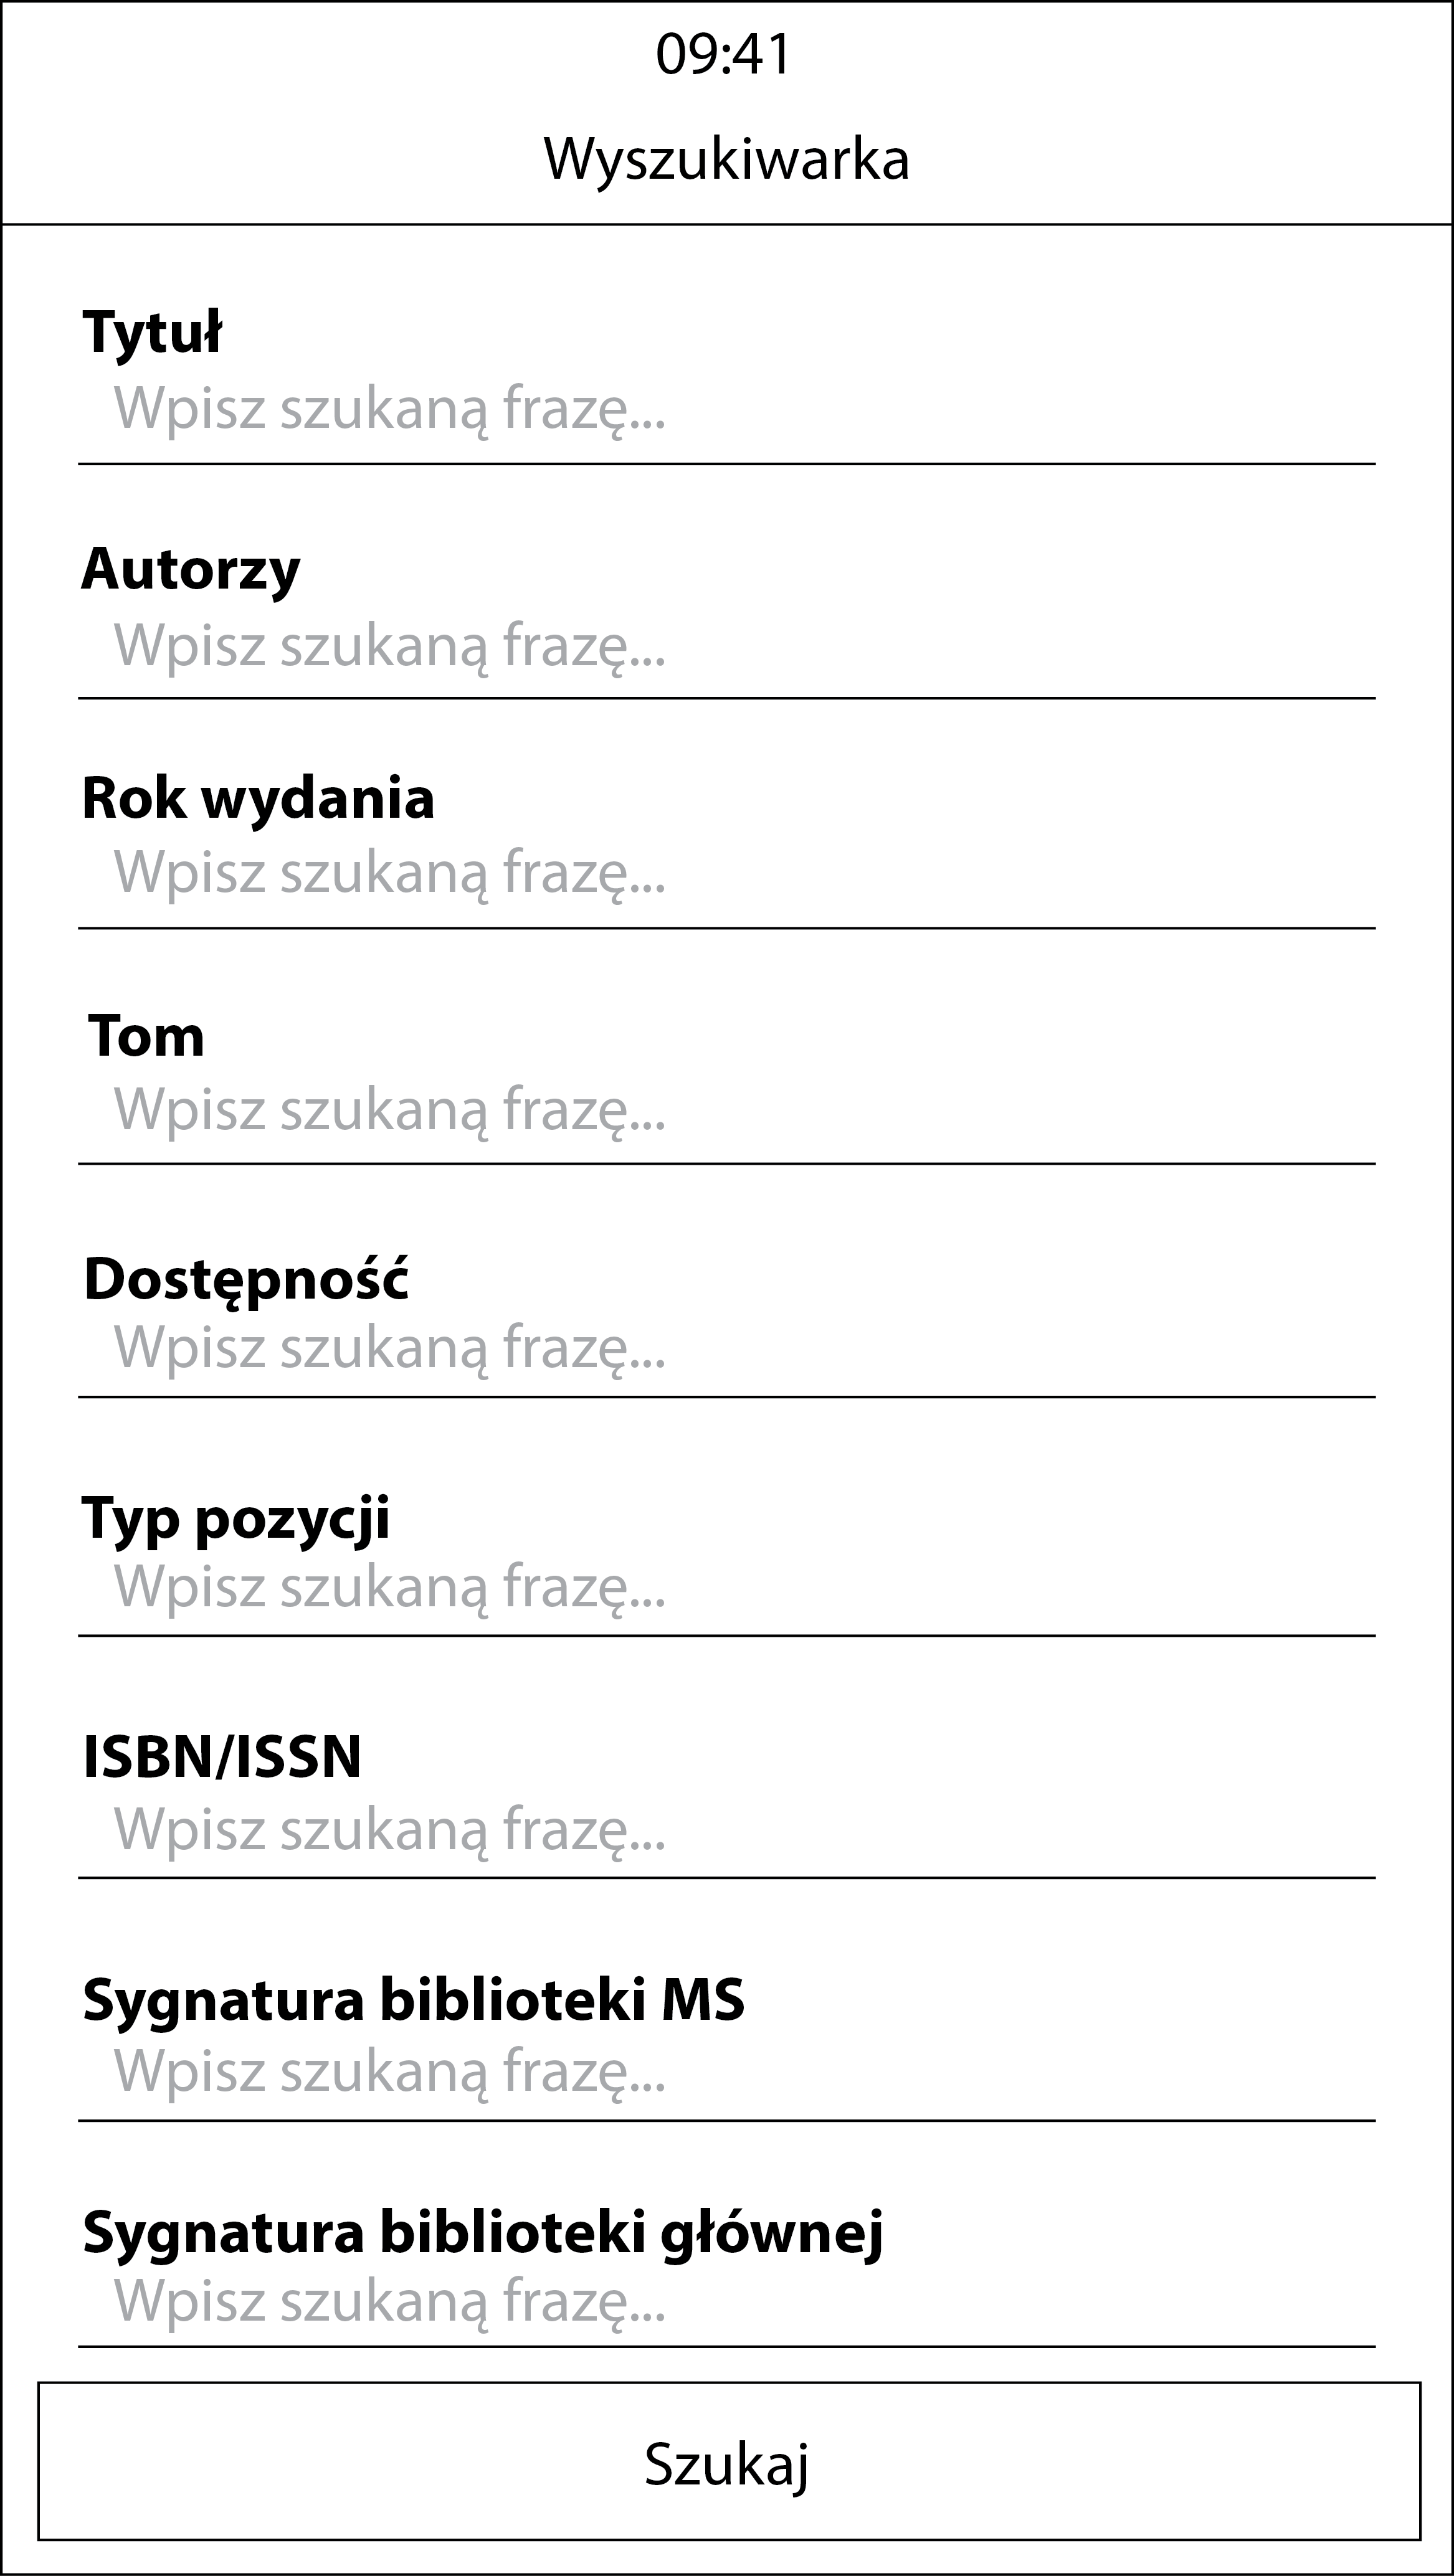
\includegraphics[width=0.4\linewidth]{img/SearchProject.png}
  \caption{Projekt ekranu wyszukiwania książek}
  \label{fig:iosCategories}
\end{figure}

Obiekt klasy tego typu jest obiektem pozwalającym przygotować formularz, który następnie będzie użyty w celu wyszukania książki w systemie biblioteki. Składa się on z natywnego elementu tabeli \verb`UITableView`, dwóch rodzajów komórek: \verb`SearchTextTableViewCell` i \verb`SearchCategoryTableViewCell` oraz z przycisku typu \verb`LoadingButton`, który został zaimplementowany na potrzeby projektu. Klasa \verb`SearchViewController` implementuje delegaty obu tych komórek:
\begin{itemize}
\item \verb`SearchTextTableViewCellDelegate` -- w celu odczytania tekstu z komórki i~zapisania odczytanego ciągu znaków w celu użycia go do wyszukiwania
\item \verb`SearchCategoryTableViewCellDelegate` -- w celu przekazania możliwości otwarcia widoku z kategoriami, po naciśnięciu przycisku 
\end{itemize}

Widok typu \verb`SearchCategoryTableViewCell` posiada możliwość uzupełniania danych przez użytkownika. Powoduje to wysunięcie się klawiatury, która niekiedy zakrywa pole, w które użytkownik wpisuje tekst. Z tego powodu został on wyposażony w rozszerzenie, które pozwala na podwijanie się widoku podczas wysuwania na nim klawiatury.

\begin{verbatim}
extension SearchViewController {
    @objc func keyboardWillShow(notification:NSNotification){
        var userInfo = notification.userInfo!
        var keyboardFrame:CGRect =
        (userInfo[UIKeyboardFrameEndUserInfoKey] as! NSValue)
        .cgRectValue
        keyboardFrame = self.view.convert(keyboardFrame, from: nil)
        tableView.contentInset =
        UIEdgeInsetsMake(0.0, 0.0,
            keyboardFrame.size.height + 8.0, 0.0)
    }
    @objc func keyboardWillHide(notification:NSNotification){
        var userInfo = notification.userInfo!
        var keyboardFrame:CGRect =
        (userInfo[UIKeyboardFrameEndUserInfoKey] as! NSValue)
        .cgRectValue
        keyboardFrame = self.view.convert(keyboardFrame, from: nil)
        tableView.contentInset =
        UIEdgeInsetsMake(0.0, 0.0,
            DefaultValues.EDGE_INSET_BOTTOM, 0.0)
    }
}
\end{verbatim}

Powyższe metody w celu monitorowania zachowania klawiatury są dodane do centrum notyfikacji w aplikacji jako obserwatory pokazania/ukrycia się natywnej klawiatury.

\begin{verbatim}
private func initObservers() {
        NotificationCenter.default.addObserver(self,
            selector: #selector(keyboardWillShow),
            name: NSNotification.Name.UIKeyboardWillShow,
            object: nil)
        NotificationCenter.default.addObserver(self,
            selector: #selector(keyboardWillHide),
            name: NSNotification.Name.UIKeyboardWillHide,
            object: nil)
    }
\end{verbatim}

Widok posiada u dołu przycisk szukania, który odpytuje usługę za pomocą spreparowanego obiektu klasy \verb`Book` utworzonego na podstawie uzupełnionych pól przez użytkownika.

W pasku nawigacji widoku, zostały podpięte dwa przyciski. Jeden z nich znajduje się po lewej stronie i służy do pobrania typów pozycji, dostępności oraz kategorii książek w przypadku braku internetu przy włączaniu aplikacji. Kliknięcie tego przycisku powoduje także wyświetlenie dialogu informującego użytkownika o pobieraniu danych. Do utworzenia dialogu została wykorzystana biblioteka JGProgressHUD \cite{JGProgressHUD}. Drugi z przycisków znajduje się po prawej stronie i służy do wyczyszczenia formularza ze wszystkich wpisanych danych.


\subsubsection{CategoriesViewController}

\begin{figure}[h]
  \centering
  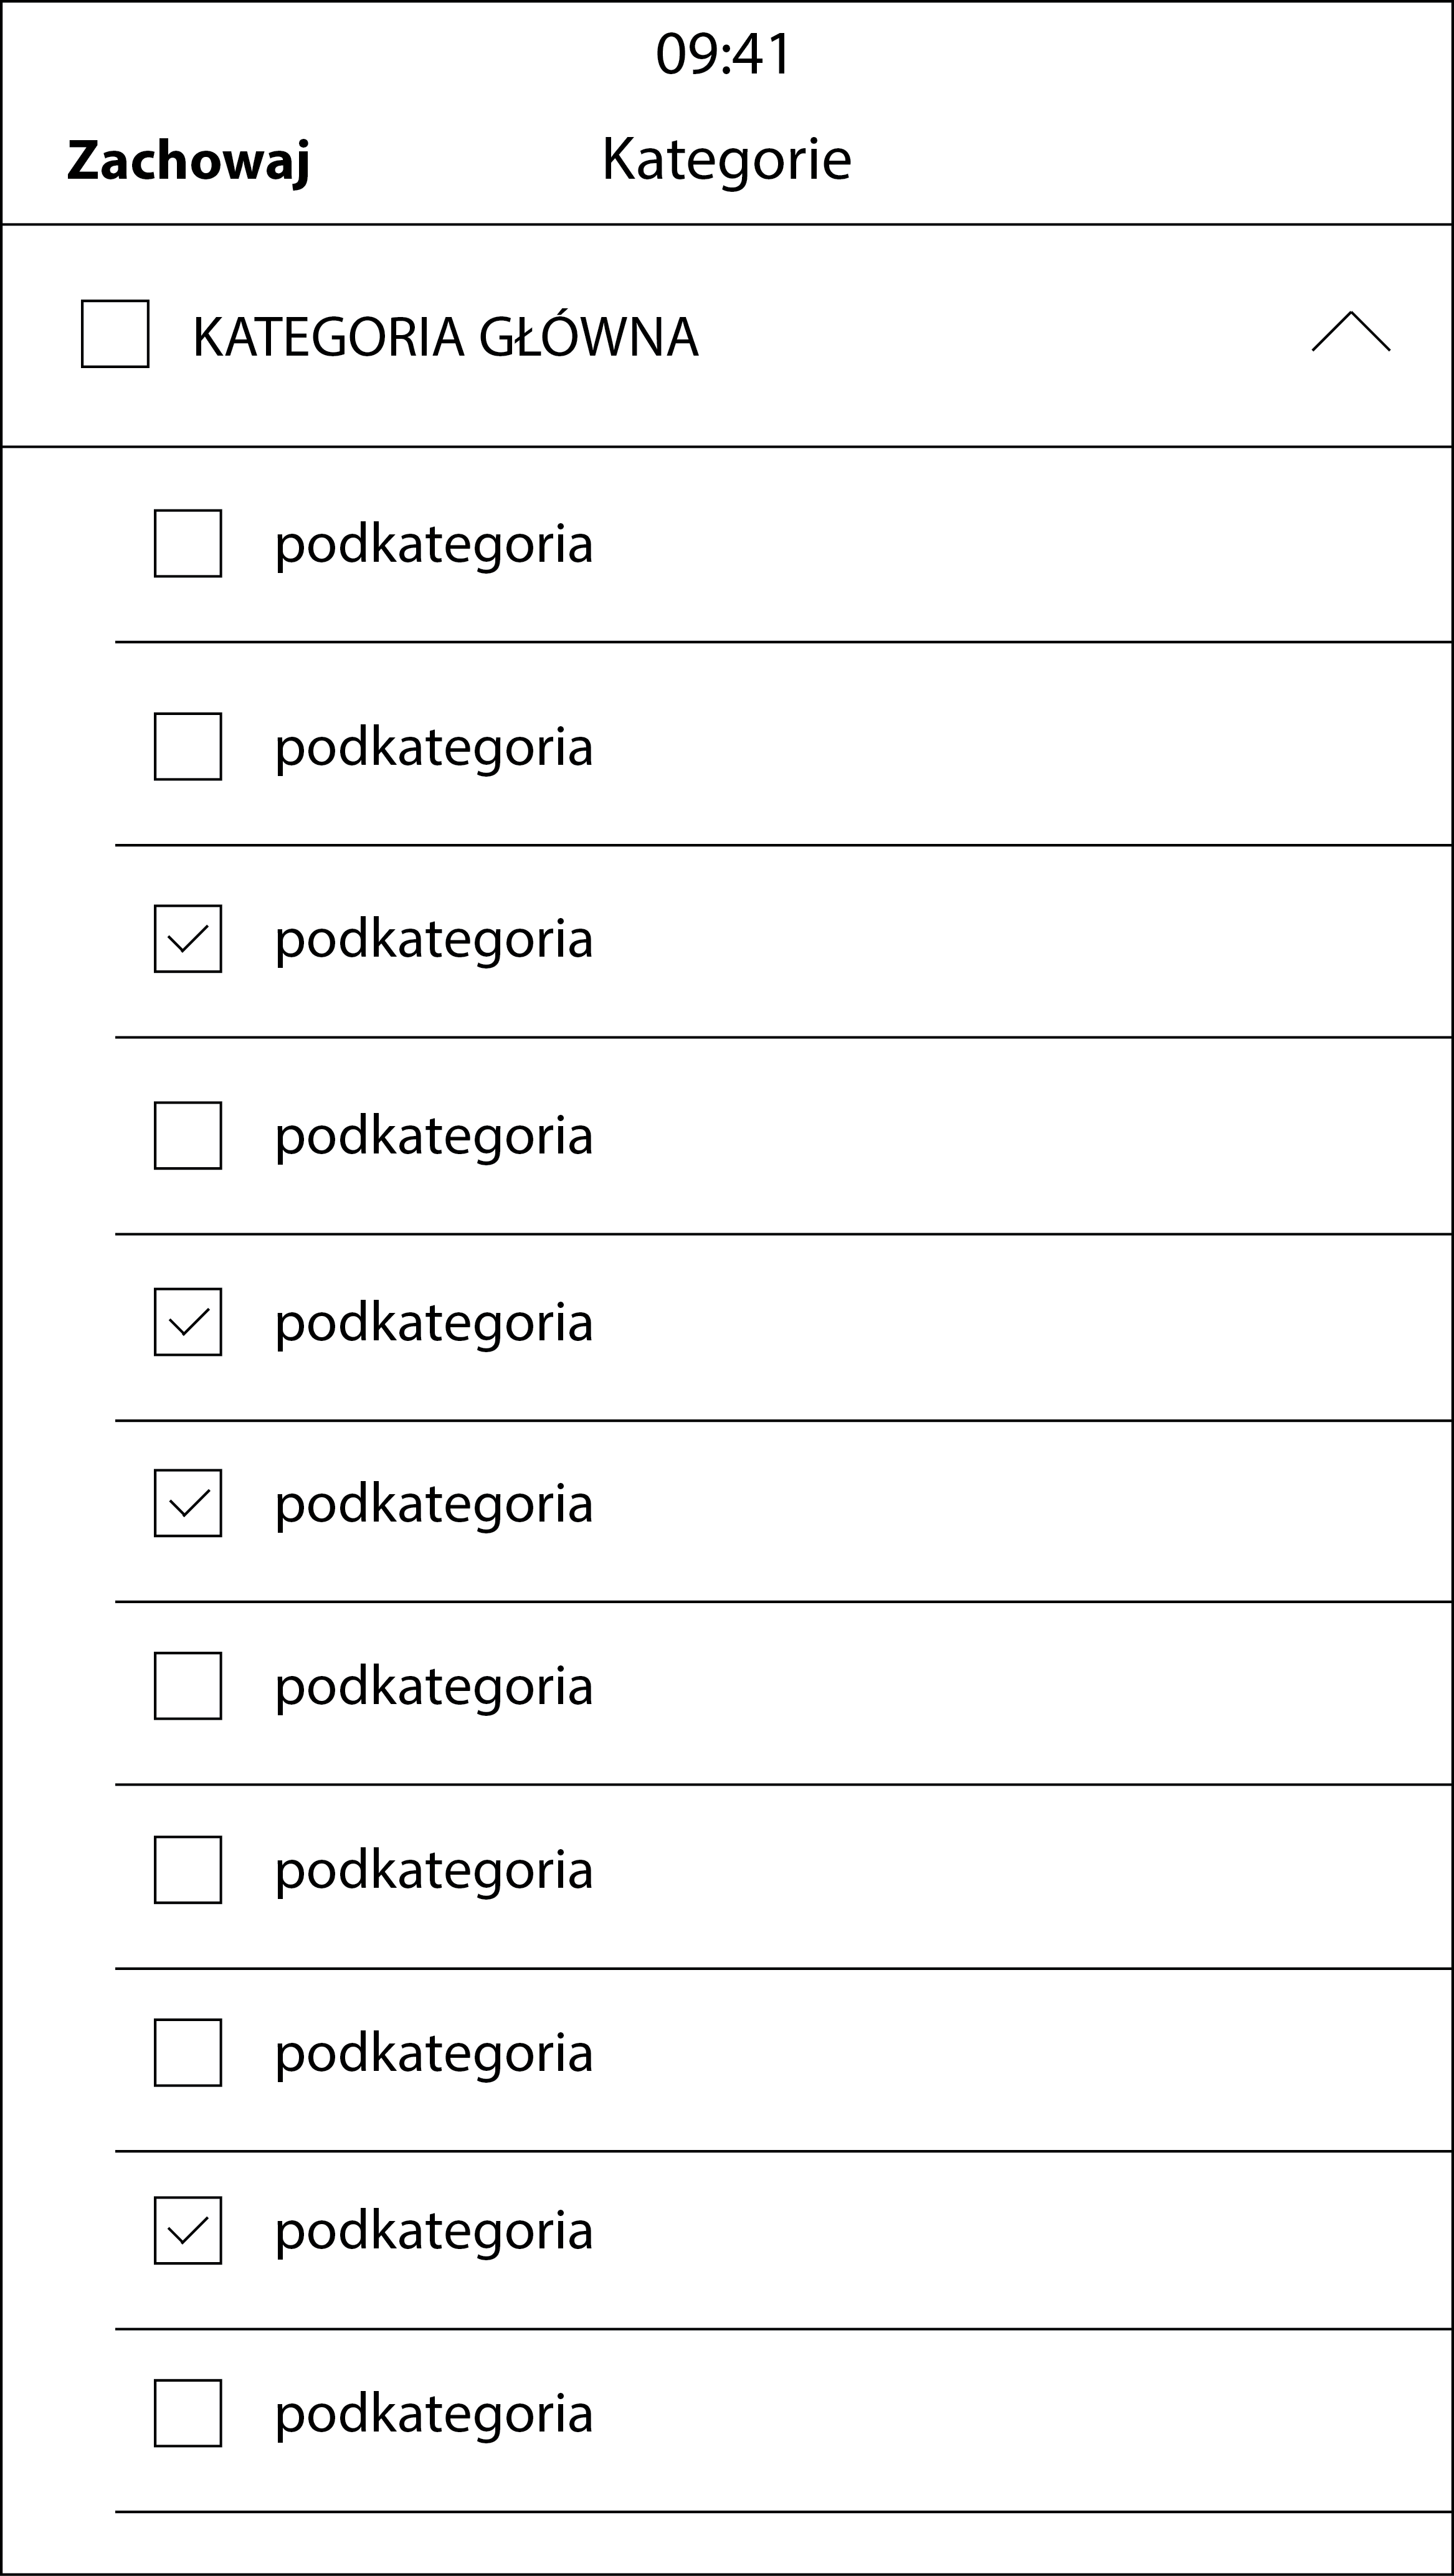
\includegraphics[width=0.4\linewidth]{img/CategoriesProject.png}
  \caption{Projekt ekranu wyboru kategorii}
  \label{fig:iosCategories}
\end{figure}

Kolejnym widokiem jest obiekt klasy \verb`CategoriesViewController`. Jest to widok posiadający komponent \verb`UITableView`, jednak w bardziej skomplikowanej konfiguracji niż widok \verb`SearchViewController`. W tabeli został zarejestrowany model komórki kategorii \verb`CategoryTableViewCell` oraz model nagłówka głównej kategorii \verb`MainCategoryHeaderView`. Tabela została stworzona jako tabela rozwijalna, tzn. po wyborze sekcji, wyświetlane są komórki do niej należące. Z powodu braku natywnego rozwiązania na tę funkcjonalność, została ona stworzona samodzielnie.

Widok posiada zmienną \verb`expandedHeaders`, która z początku jest wypełniona wartościami typu \verb`false`.
\begin{verbatim}
var expandedHeaders: [Bool] = []
...
func collapseAllHeaders() {
    let mainCategoriesCount =
        SessionManager.shared.mainCategories.count
    expandedHeaders =
        Array(repeating: false, count: mainCategoriesCount)
}
\end{verbatim}
Indeks każdego elementu tabeli odzwierciedla sekcję nagłówka. Pozwala to stwierdzić, które z sekcji są rozwinięte, a które zwinięte. Kliknięcie w przycisk rozwijania sekcji, uruchamia metodę ze specjalnie stworzonego na te potrzeby protokołu obsługującego nagłówek.
\begin{verbatim}
extension CategoriesViewController: MainCategoryHeaderViewDelegate {
    ...
    func expandSubcategories(
        usingHeader header: MainCategoryHeaderView)
    {
        var headerIsExpanded = expandedHeaders[header.section]
        headerIsExpanded = !headerIsExpanded
        header.isExpanded = headerIsExpanded
        expandedHeaders[header.section] = headerIsExpanded
        tableView.reloadData()
    }
}
\end{verbatim}
Powoduje ona przestawienie odpowiedniej wartości w tablicy \verb`expandedHeaders` na przeciwną, przekazanie jej do widoku i odświeżenie tabeli. Natywne metody delegatowe klasy \verb`UITableView` zostały uzupełnione w sposób obsługujący informacje dotyczące rozwiniętej/zwiniętej sekcji. Implementacja metody odpowiadającej za ilość wierszy, pochodząca z protokołu \verb`UITableViewDataSource` została zaprezentowana poniżej.
\begin{verbatim}
func tableView(_ tableView: UITableView,
    numberOfRowsInSection section: Int) -> Int
{
    if expandedHeaders[section] {
        return SessionManager.shared.mainCategories[section]
            .subcategories.count
    } else {
        return 0
    }
}
\end{verbatim}
W przypadku rozwiniętej sekcji zwraca ilość wierszy równą ilości podkategorii należących do kategorii głównej z danej sekcji. Dla zwiniętego nagłówka nie wyświetla żadnego wiersza.

Opisywany widok obsługuje także możliwość wyboru wierszy bądź nagłówków, w celu późniejszego wykorzystania wybranych kategorii. W tym celu również zostały wykorzystane zmienne służące do pamiętania stanu wyboru.
\begin{verbatim}
var selectedHeaders: [Bool] = []
var selectedCells: [IndexPath:Bool] = [:]
\end{verbatim}
Przedstawiają one zaznaczone nagłówki (obiekt typu \verb`Array`) oraz zaznaczone komórki (obiekt typu \verb`Dictionary`). Każde wybranie nagłówka, zmienia jego stan, jednocześnie wpływając na stan komórek należących do danej sekcji. Wybór nagłówka powoduje skorzystanie z metody przypisującej w słowniku \verb`selectedCells` zmienne typu \verb`Bool` do obiektów typu \verb`IndexPath`, które określają pozycję komórki w tabeli. Jednocześnie przypisując obiekty, komórki w zadanych pozycjach są zaznaczane lub odznaczane.

Nie tylko nagłówek może wpłynąć na stan komórki. Istnieje również odwrotna zależność. Wybór komórek także może wpłynąć na stan nagłówka (na przykład w~przypadku zaznaczenia wszystkich podkategorii). Obsługa tego zdarzenia została opisana poniższą metodą.
\begin{verbatim}
private func trySelectHeader(inSection section: Int) {
    let subcategories = SessionManager.shared
        .mainCategories[section].subcategories
    if subcategories.isEmpty { return }
    for (index, _) in subcategories.enumerated() {
        let indexPath = IndexPath(row: index, section: section)
        guard let selected = selectedCells[indexPath]
        else { return }
        if !selected {
            toggleHeader(inSection: indexPath.section,
                select: false)
            return
        }
    }
    toggleHeader(inSection: section, select: true)
}
\end{verbatim}

Dodatkowo obiekt typu \verb`CategoriesViewController` obsługuje zapis wybranych kategorii jak i załadowanie zaznaczonych już wcześniej kategorii, zaraz po wejściu na widok. 


\subsubsection{BookListViewController}

\begin{figure}[h]
  \centering
  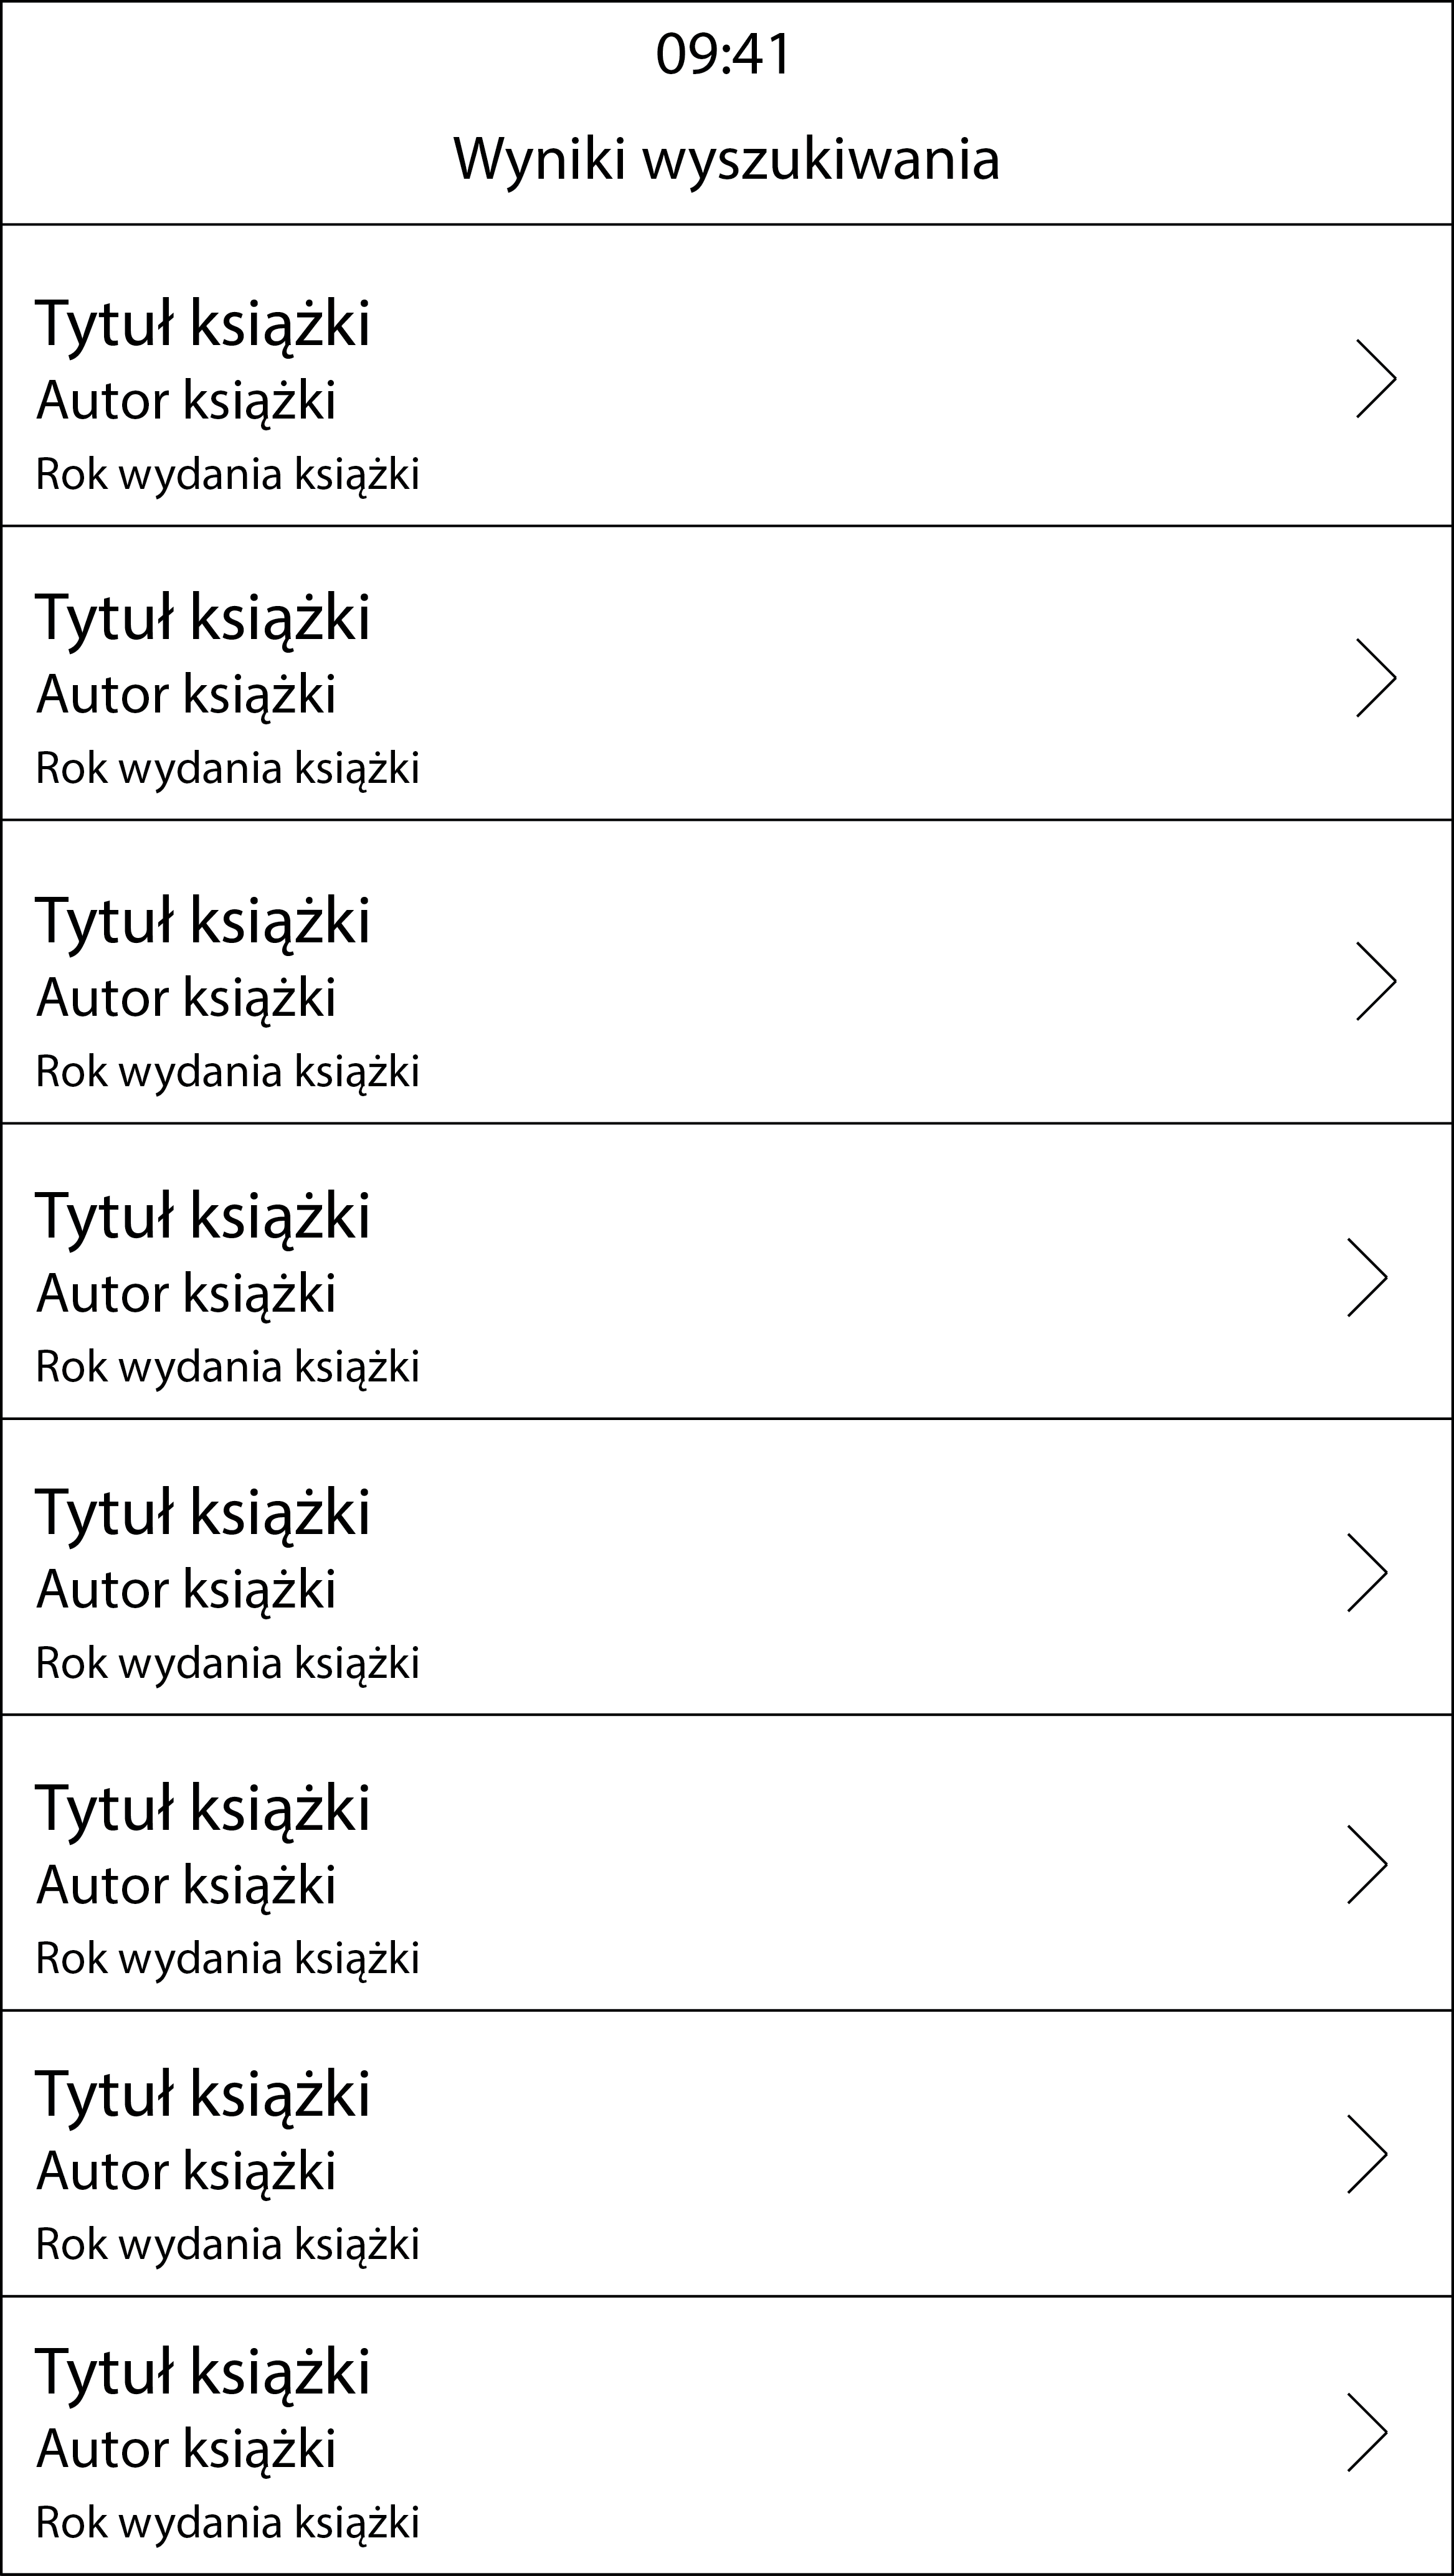
\includegraphics[width=0.4\linewidth]{img/BookListProject.png}
  \caption{Projekt ekranu listy książek}
  \label{fig:iosCategories}
\end{figure}

Obiekt klasy \verb`BookListViewController` jest następnym z widoków posiadających tabelę \verb`UITableView`. Służy do wyświetlania wyników wyszukiwania. Została w~nim zarejestrowana komórka typu \verb`BookTableViewCell`, która wyświetla tytuł oraz autora znalezionej książki. Tabela została przystosowana w taki sposób, aby wyświetlać pewną ilość książek, a w przypadku zaistniałej potrzeby, dociągać kolejną ich ilość. Metoda \verb`tryFetchMoreBooks(loadedIndexPath: IndexPath)`, która została zaimplementowana, jest wywoływana przy każdym ładowaniu się komórki na widoku. W przypadku, gdy ładowana jest szósta od końca komórka, metoda ta odpytuje usługę o kolejne książki. Gdy je otrzyma, dopisuje je do tablicy książek co powoduje odświeżenie widoku, ze zwiększoną liczbą znalezionych pozycji.

\begin{verbatim}
fileprivate func tryFetchMoreBooks(loadedIndexPath: IndexPath) {
    let rowWhenFetchNeeded = books.count - 5
    if loadedIndexPath.row == rowWhenFetchNeeded && canFetchMore {
        offset += DefaultValues.BOOKS_PER_FETCH
        RequestManager.shared.getBooks(
            withOffset: offset,
            completion: appendFetchedBooks)
    }
}
fileprivate func appendFetchedBooks(_ fetchedBooks: [Book]) {
    if fetchedBooks.isEmpty {
        canFetchMore = false
        return
    }
    self.books.append(contentsOf: fetchedBooks)
}
\end{verbatim}

Widok przedstawiający listę książek, obsługuje dodatkowo natywne rozwiązanie typu \textit{3D Touch}. Pozwala ono na podgląd zawartości komórki oraz wykonanie dodatkowych akcji przed jej wyborem. W tym celu, zostało stworzone rozszerzenie klasy \verb`BookListViewController` obsługujące akcje mocnego przyciśnięcia wiersza (\textit{Peek}) oraz jego jeszcze mocniejszego dociśnięcia (\textit{Pop}).

\begin{verbatim}
extension BookListViewController: UIViewControllerPreviewingDelegate {
    //PEEK
    func previewingContext(
        _ previewingContext: UIViewControllerPreviewing,
        viewControllerForLocation location: CGPoint) -> UIViewController?
    {
        guard let indexPath = tableView.indexPathForRow(at: location),
            let cell = tableView.cellForRow(at: indexPath)
        else {
            return nil
        }
        let book = books[indexPath.row]
        let detailsVC = getBookDetailsViewController(forBook: book)
        previewingContext.sourceRect = cell.frame
        return detailsVC
    }
    //POP
    func previewingContext(
    _ previewingContext: UIViewControllerPreviewing,
    commit viewControllerToCommit: UIViewController) {
        let navigationController = UINavigationController(
            rootViewController: viewControllerToCommit)
        self.showDetailViewController(navigationController,
            sender: self)
    }
}
\end{verbatim}
Akcja \textit{3D Touch} jest obsługiwana jedynie na telefonach typu iPhone 6s i nowszych. Z~tego powodu należy po załadowaniu widoku upewnić się, czy jest sens rejestrowania metod szybkiego podglądu.
\begin{verbatim}
override func viewDidAppear(_ animated: Bool) {
    super.viewDidAppear(animated)
    if traitCollection.forceTouchCapability == .available {
        registerForPreviewing(with: self, sourceView: tableView)
    }
}
\end{verbatim}

Widok typu \verb`BookListViewController` posiada dodatkowo obsługę w przypadku, gdy ilość otrzymanych książek z usługi jest równa 0. Do obsługi pustego ekranu wykorzystana została biblioteka \textit{UIEmptyState} \cite{UIEmptyState}. Jest to mało rozpowszechniona biblioteka służąca do analizowania wyświetlanych informacji w tabeli \verb`UITableView` lub kolekcji \verb`UICollectionView`, która w przypadku liczby elementów do wyświetlenia równej 0, pokaże użytkownikowi dowolnie spersonalizowaną informację o braku danych do zaprezentowania.

Biblioteka ta jest napisana w stosunkowo przyjazny sposób dla programisty. W celu zastosowania jej funkcjonalności, należy zaimplementować dwa typy protokołów: \verb`UIEmptyStateDelegate` oraz \verb`UIEmptyStateDataSource`. Następnie można przejść do przypisywania potrzebnych zmiennych, które zostaną automatycznie wyświetlone w przypadku braku elementów do wyświetlenia na widoku.
\begin{verbatim}
extension BookListViewController:
    UIEmptyStateDelegate, UIEmptyStateDataSource
{
    fileprivate func setEmptyStateDelegates() {
        self.emptyStateDelegate = self
        self.emptyStateDataSource = self
    }
    var emptyStateBackgroundColor: UIColor {
        return .main
    }
    var emptyStateTitle: NSAttributedString {
        let title = R.string.localizable.noResults()
        let range = (title as NSString).range(of: title)
        let titleAttributedString =
            NSMutableAttributedString(string: title)
        let titleColor = UIColor.tintDark
        titleAttributedString.addAttribute(
            NSAttributedStringKey.foregroundColor,
            value: titleColor, range: range)
        return titleAttributedString
    }
    var emptyStateImage: UIImage? {
        let image = R.image.bookShelf()
            .maskWithColor(color: .tintDark)
        return image
    }
}
\end{verbatim}


\subsubsection{BookDetailsViewController}

\begin{figure}[h]
  \centering
  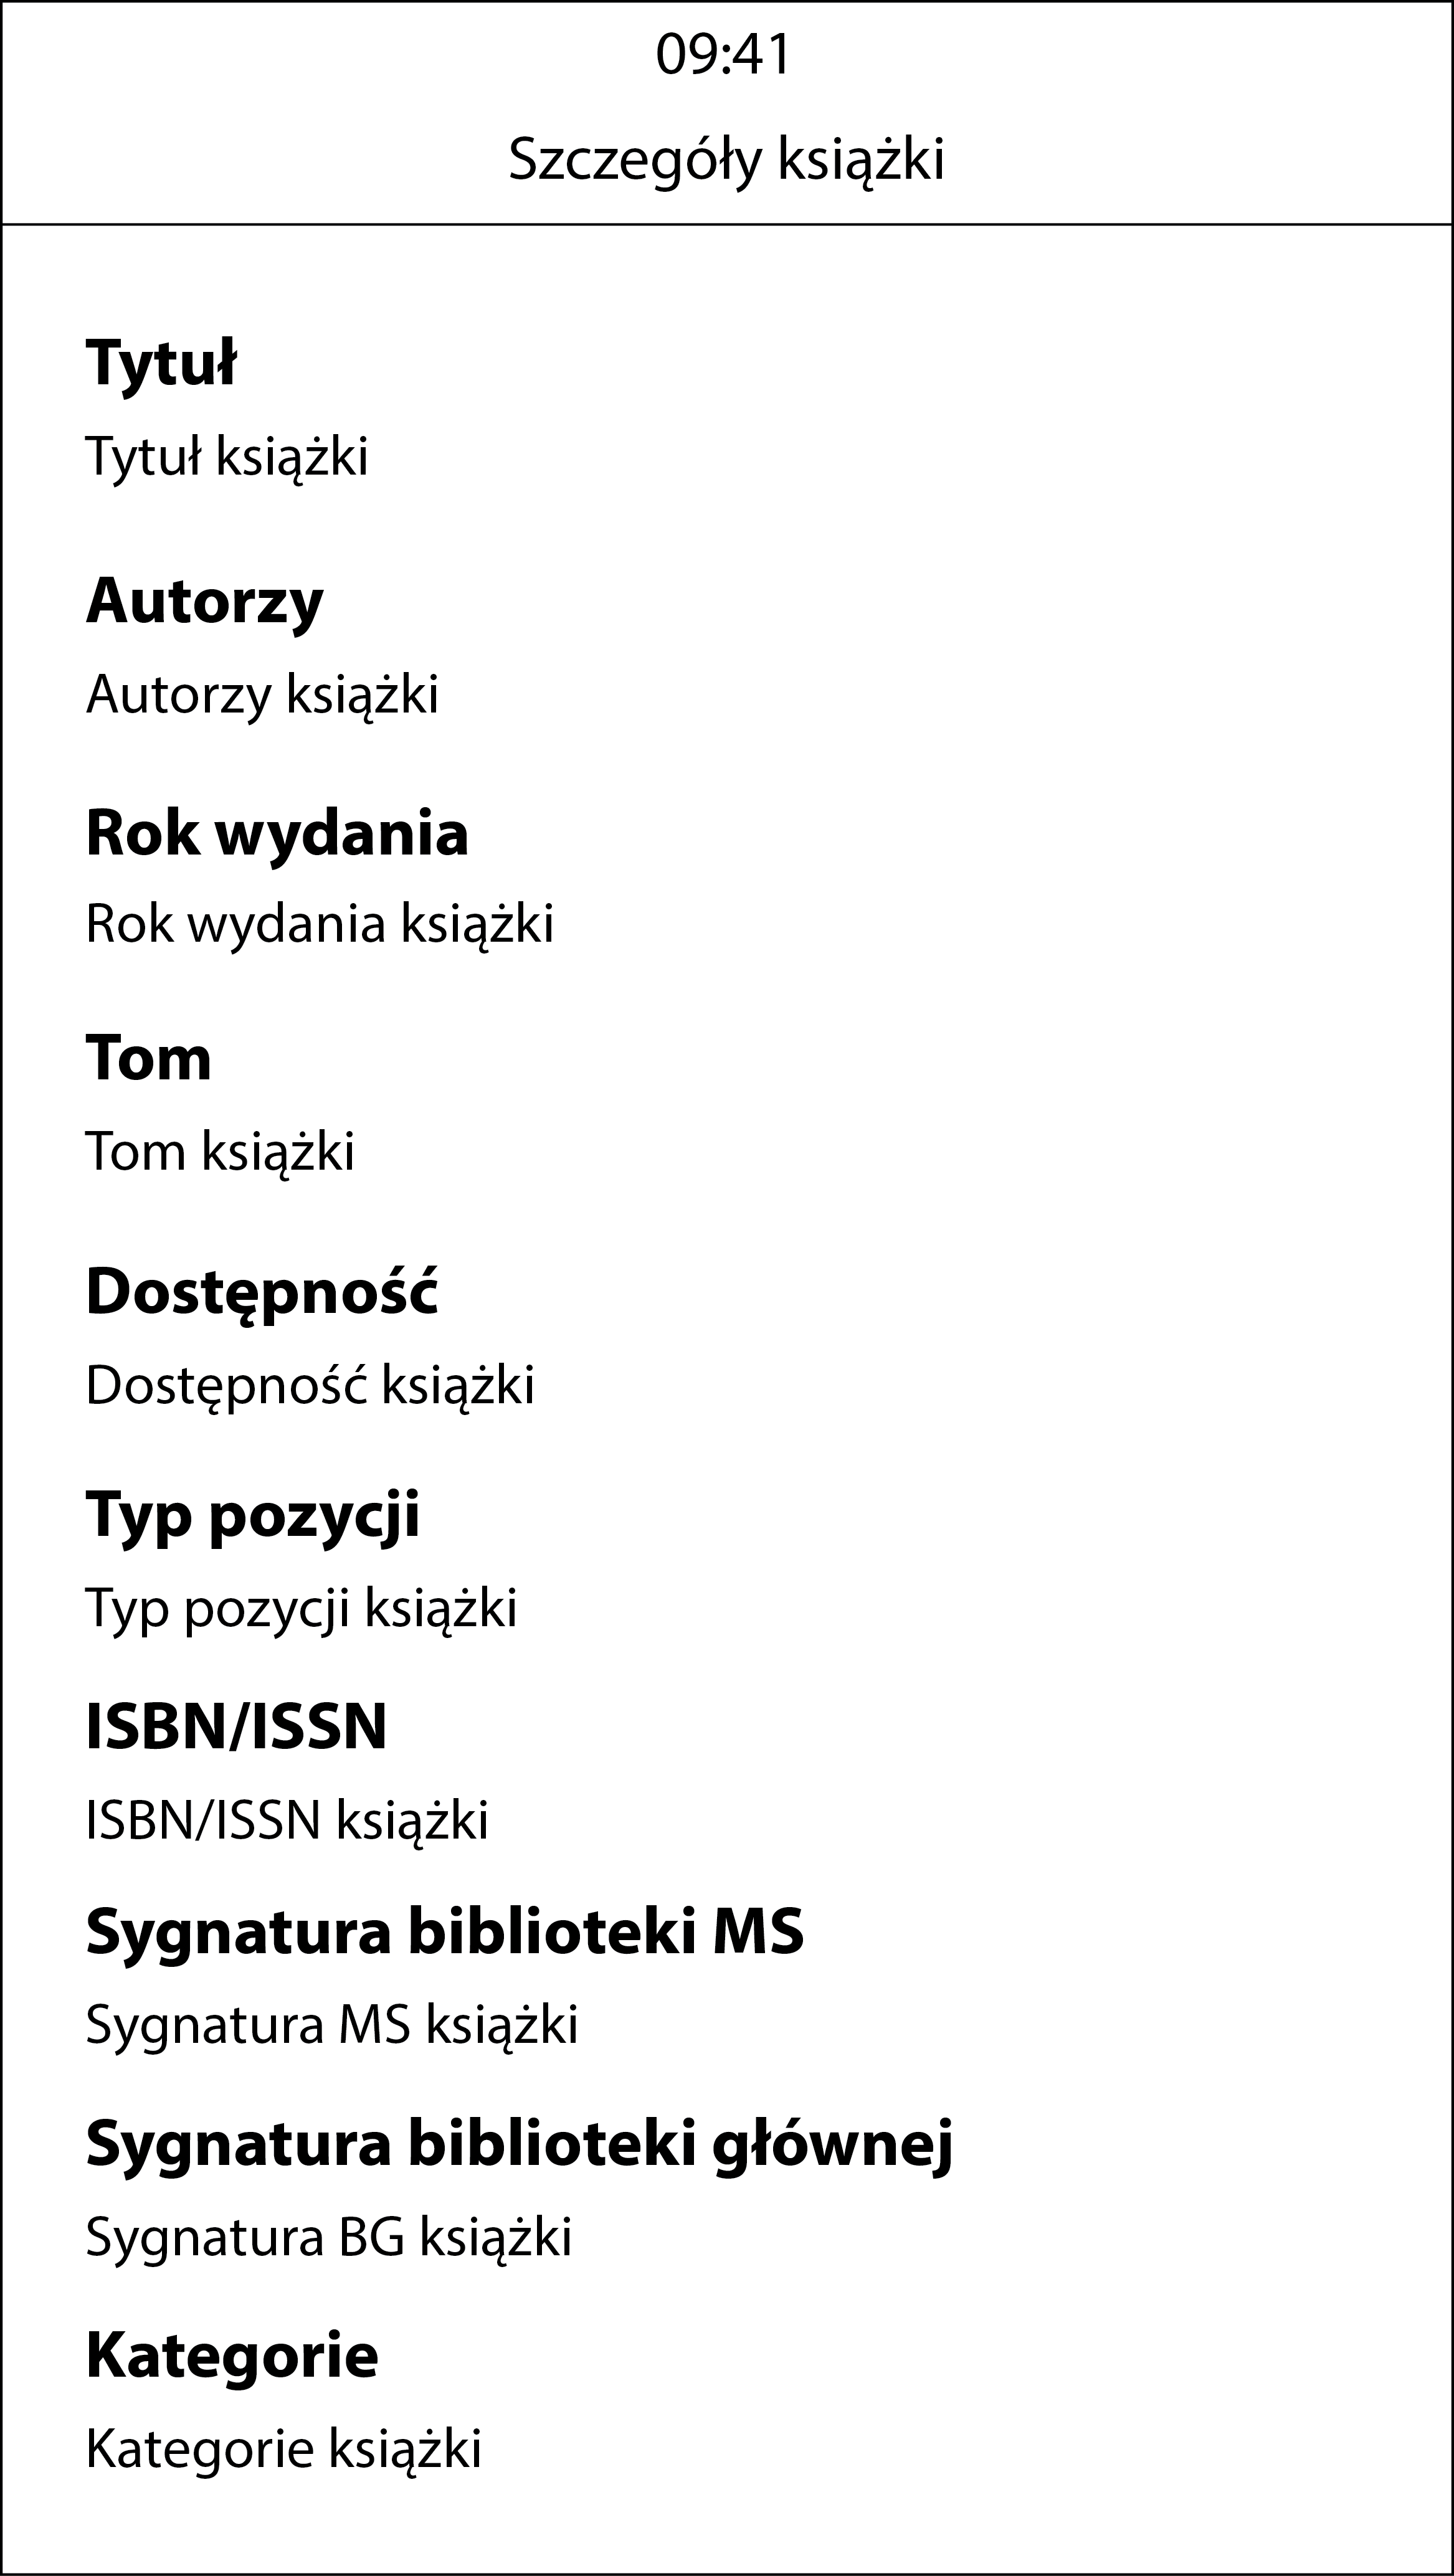
\includegraphics[width=0.4\linewidth]{img/DetailsProject.png}
  \caption{Projekt ekranu szczegółów książki}
  \label{fig:iosCategories}
\end{figure}

Klasa \verb`BookDetailsViewController` przedstawia obiekt widoku informacji o książce. Składa się ona tak jak inne widoki z tabeli \verb`UITableView`, a do wyświetlenia zawartości wykorzystuje komórkę typu \verb`BookDetailTableViewCell` posiadająca jedynie tytuł oraz zawartość pola opisującego książkę. Opisywana klasa widoku, jest dużo prostsza od poprzednich. Elementem wyróżniającym ją spośród pozostałych, jest zmienna typu \verb`[UIPreviewActionItem]`, która odpowiada za szybkie akcje w~trybie \textit{Peek}, będąc na poprzednim widoku typu \verb`BookListViewController`.
\begin{verbatim}
override var previewActionItems: [UIPreviewActionItem] {
    let copyTitleAction = UIPreviewAction(
        title: R.string.localizable.copyTitle(),
        style: .default) {
            (action, vc) in
            UIPasteboard.general.string = self.book?.bookTitle
    }
    let copyAuthorAction = UIPreviewAction(
        title: R.string.localizable.copyAuthor(),
        style: .default) {
            (action, viewcontroller) in
            UIPasteboard.general.string = self.book?.bookAuthors
    }
    return [copyTitleAction, copyAuthorAction]
}
\end{verbatim} 


\subsubsection{SessionManager}

\verb`SessionManager` to klasa odpowiadająca za zarządzanie, przechowywanie i udostępnianie danych do widoków podczas jednej sesji działania aplikacji. Klasa ta posiada trzy pola. Wystarczają one do zarządzania całą sesją, która jest aktywna, dopóki aplikacja znajduje się w pamięci RAM urządzenia.
\begin{itemize}
\item \verb`var searchedBook: Book!` -- pole odpowiadające za przetrzymywanie szablonowej, poszukiwanej przez użytkownika książki. Pole to jest aktualizowane z~każdą zmianą użytkownika na widoku wyszukiwania.
\item \verb`var mainCategories: [MainCategory]` -- wszystkie kategorie (główne wraz z podkategoriami) zaciągnięte z usługi po wejściu w aplikację.
\item \verb`var dictionaryTypes: DictionaryTypes!` -- wszystkie możliwe typy pozycji oraz stany dostępności książek. Otrzymywane są z usługi po otwarciu aplikacji.
\end{itemize}


Klasa \verb`SessionManager`, z powodu zarządzania całą sesją, została zaimplementowana z zastosowaniem wzorca projektowego Singleton. Zgodnie z jego założeniami, klasa posiada statyczną instancję oraz prywatny konstruktor.
\begin{verbatim}
class SessionManager {
    private init() {
        searchedBook = Book()
        dictionaryTypes = DictionaryTypes()
    }
    static let shared = SessionManager()
    ...
}
\end{verbatim}


\subsubsection{RequestManager}

Za odpytywanie usługi odpowiada klasa \verb`RequestManager`. Klasa ta jest również Singletonem. Jest ona napisana korzystając jedynie z natywnych rozwiązań języka \textit{Swift 4}. Dzięki implementacji odpowiednich protokołów przez klasy modelowe, metoda ta jest w stanie bezpośrednio stworzyć obiekt z danych, które przyszły z usługi w formacie \textit{.json}. Poniżej został przedstawiony przykład zaciągania z usługi obiektu tablicy wszystkich kategorii głównych.
\begin{verbatim}
func getCategories(completion: @escaping (([MainCategory])->())) {
    guard let request = getRequest(usingHttpMethod: "GET",
        forEndpoint: CATEGORY_ENDPOINT) else { return }
    URLSession.shared.dataTask(with: request) {
        (data, response, error) in
        if let error = error {
            NSLog(error.localizedDescription)
        }
        guard let data = data else { return }
        do {
            let mainCategories = try
                JSONDecoder().decode([MainCategory].self, from: data)
            completion(mainCategories)
        } catch let jsonError {
            NSLog(jsonError.localizedDescription)
            completion([])
        }
    }.resume()
}
\end{verbatim}

Każda z metod odpytujących usługę zaimplementowana jest korzystając z metody tworzącej typowy obiekt klasy \verb`URLRequest?`. Jest on tworzony na podstawie typu metody (w przypadku naszego projektu korzystamy jedynie z typów \textit{GET} oraz \textit{POST}) oraz końcówki adresu do którego powinno zostać wysłane zapytanie.
\begin{verbatim}
fileprivate func getRequest(
    usingHttpMethod httpMethod: String?,
    forEndpoint endpoint: String) -> URLRequest?
{
    let address = URL_STRING + endpoint
    guard let url = URL(string: address) else { return nil }
    var request = URLRequest(url: url)
    request.httpMethod = httpMethod
    request.setValue("application/json",
        forHTTPHeaderField: "Content-Type")
    return request
}
\end{verbatim}


\subsection{Interfejs użytkownika}


\subsubsection{Wyszukiwarka książek}

Aplikacja po uruchomieniu, przechodzi bezpośrednio do ekranu wyszukiwarki książek, jak zostało przedstawione na rysunku \ref{fig:iosSearchEmpty}. Aplikacja do poprawnego działania wymaga połączenia użytkownika z internetem. W przypadku braku połączenia internetowego, na ekranie pojawi się stosowna informacja zaraz po wejściu na widok. Przycisk w lewym górnym roku pozwala na odświeżenie zawartości. Użytkownik ma możliwość uzupełnienia dowolnych pól, w zależności od poszukiwanej przez niego pozycji. 

\begin{figure}
\centering
\begin{minipage}{.5\textwidth}
    \centering
    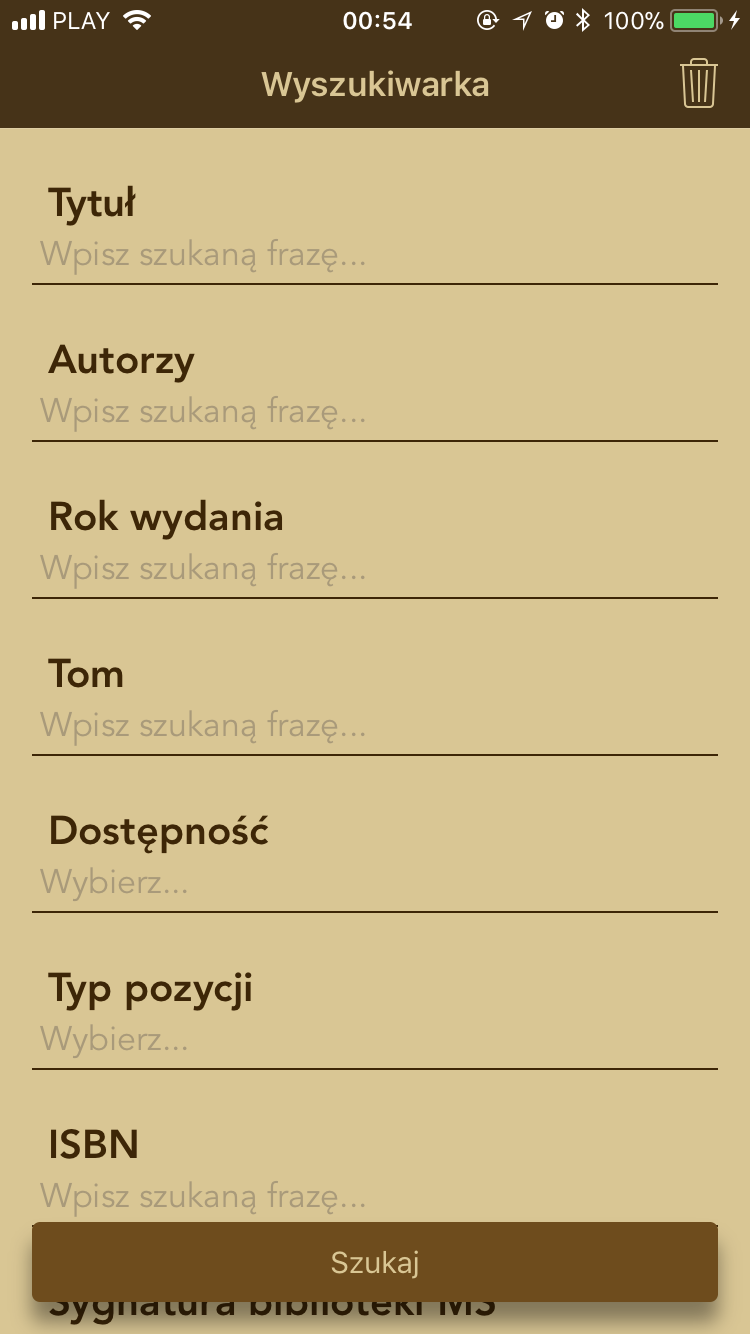
\includegraphics[width=0.8\linewidth]{img/iOS/ios1.PNG}
    \caption{Niewypełniony ekran wyszukiwania książki}
    \label{fig:iosSearchEmpty}
\end{minipage}%
\begin{minipage}{.5\textwidth}
    \centering
    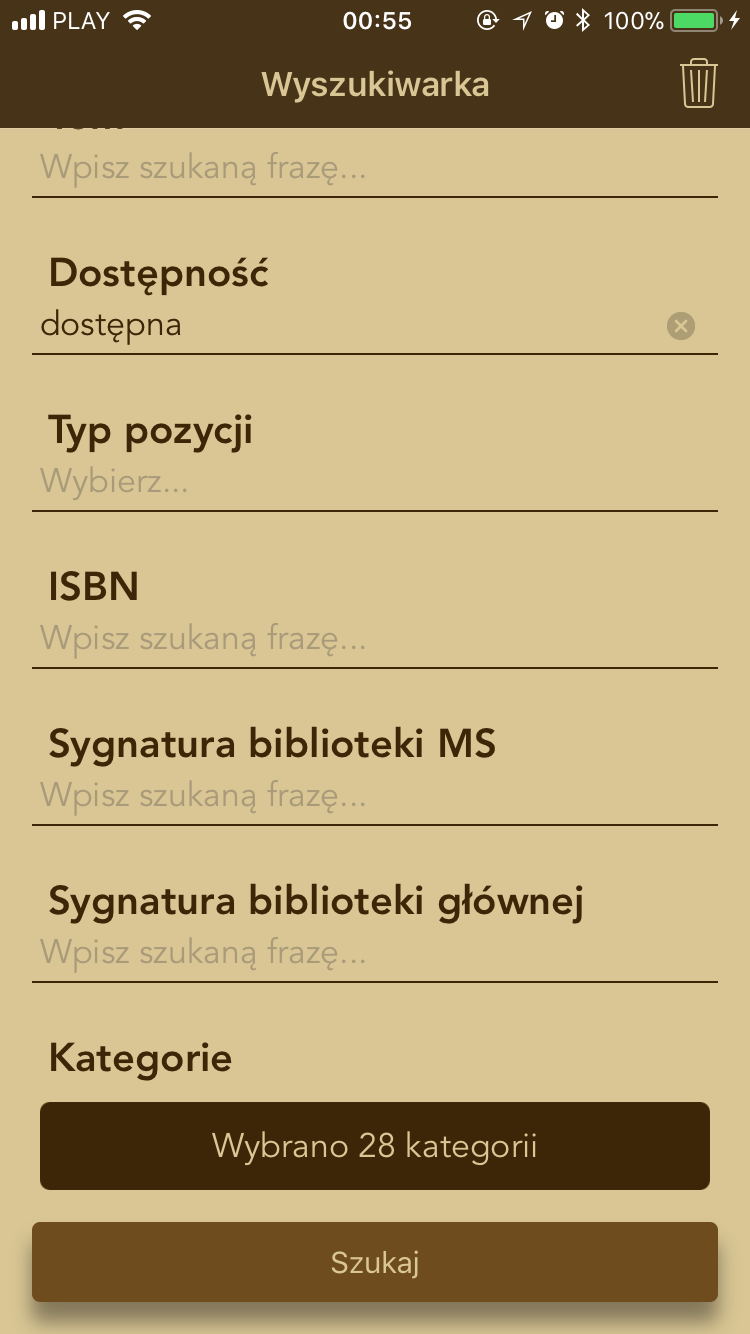
\includegraphics[width=0.8\linewidth]{img/iOS/ios3.PNG}
    \caption{Częściowo uzupełniony ekran wyszukiwania książki}
    \label{fig:iosSearchFilled}
\end{minipage}
\end{figure}

Pierwsze z pól są polami służącymi do uzupełnienia tekstu za pomocą klawiatury systemowej bądź wyboru jednego z kilku elementów z prostej listy. Ostatnia z komórek posiada przycisk przenoszący użytkownika do ekranu wyboru kategorii, jak na rysunku \ref{fig:iosCategories}. W prawym górnym rogu ekranu znajduje się przycisk, służący do wyczyszczenia wszystkich pól wyszukiwarki. Usunięcie dowolnego wypełnionego pola również jest możliwe -- wystarczy wybrać szary przycisk znajdujący się obok wypełnionego pola, jak na rysunku \ref{fig:iosSearchFilled}.

U dołu ekranu znajduje się przycisk wyszukiwania. Kliknięcie go, uruchamia wyszukiwanie, co jest oznajmione poprzez kręcące się kółeczko wewnątrz przycisku.


\subsubsection{Wybór kategorii}

Ekran kategorii, jest listą elementów posortowanych w sekcjach. Niektóre z sekcji są rozwijalne. Rozwinięcie sekcji pozwala użytkownikowi przejrzeć wszystkie podkategorie dla wybranej kategorii głównej. Użytkownik może na tym ekranie dokonać wyboru zakresu poszukiwanej przez niego książki. W przypadku wyboru kategorii głównej, zaznaczane są automatycznie wszystkie jej podkategorie. W prawym górnym rogu znajduje się przycisk z ikoną kosza. Pozwala on wyczyścić wybrane kategorie i zacząć wybór od nowa.


\begin{figure}[h]
  \centering
  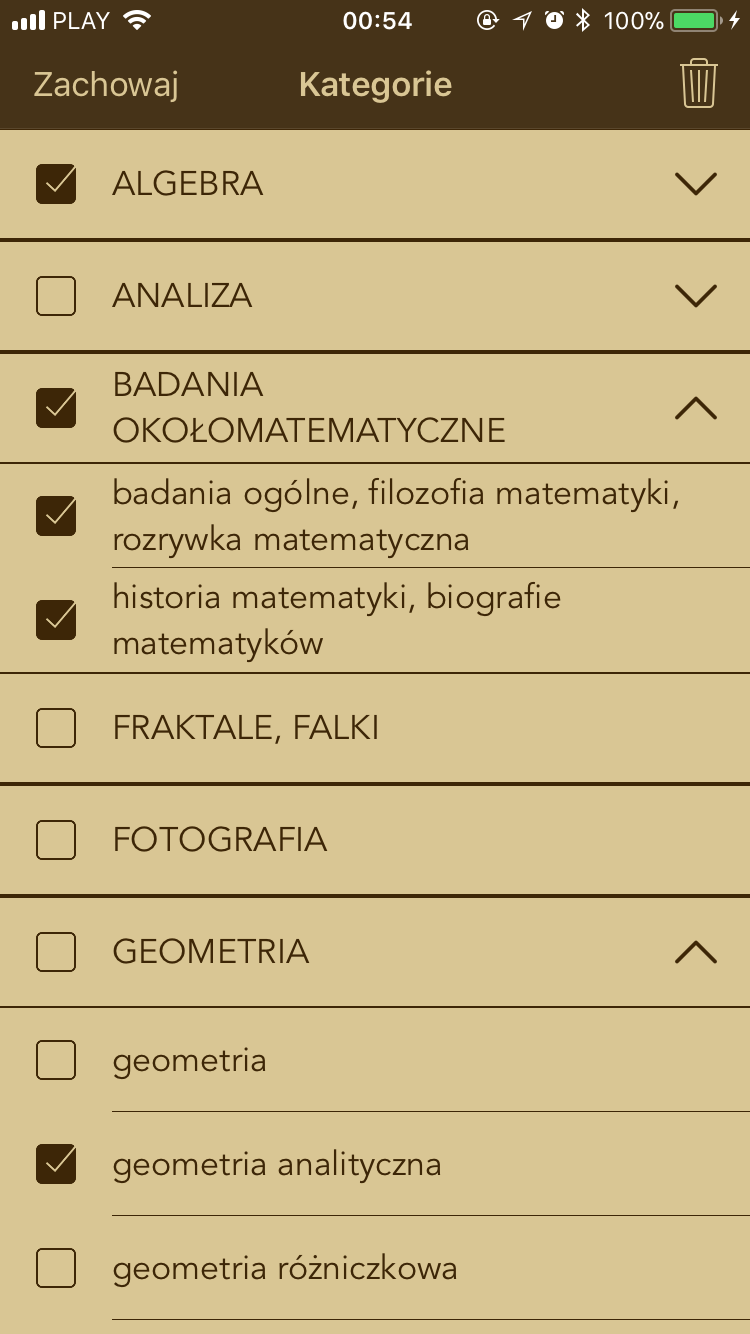
\includegraphics[width=0.4\linewidth]{img/iOS/ios2.PNG}
  \caption{Ekran wyboru kategorii}
  \label{fig:iosCategories}
\end{figure}

W lewym górnym rogu umiejscowiony jest przycisk zapisu wybranych kategorii. Jego wybór przenosi użytkownika z powrotem na ekran wyszukiwania. Po powrocie, przycisk do wyboru kategorii wyświetla ich konkretną ilość jaka została wybrana przez użytkownika. Zostało to przedstawione na rysunku \ref{fig:iosSearchFilled}.


\subsubsection{Wyniki wyszukiwania}

Na ekranie wyszukiwania, wybór przycisku odpowiadającego za szukanie, przekierowuje użytkownika do ekranu Wyników wyszukiwania. W przypadku nie znalezienia żadnej pozycji pasującej do zapytania, wyświetlany jest ekran znajdujący się na rysunku \ref{fig:iosResultsEmpty}. Ekran z rysunku numer \ref{fig:iosResults}, przedstawia listę z poprawnie znalezionymi pozycjami. Składa się on z wierszy przedstawiających tytuły oraz autorów wyszukanych pozycji. Ilość wyszukanych książek jest równa 20 lub mniejsza. W przypadku, gdy jest ona maksymalna, użytkownik może przejść do dołu listy w celu doładowania i wyświetlenia kolejnych rekordów na widoku.

\begin{figure}
\centering
\begin{minipage}{.5\textwidth}
    \centering
    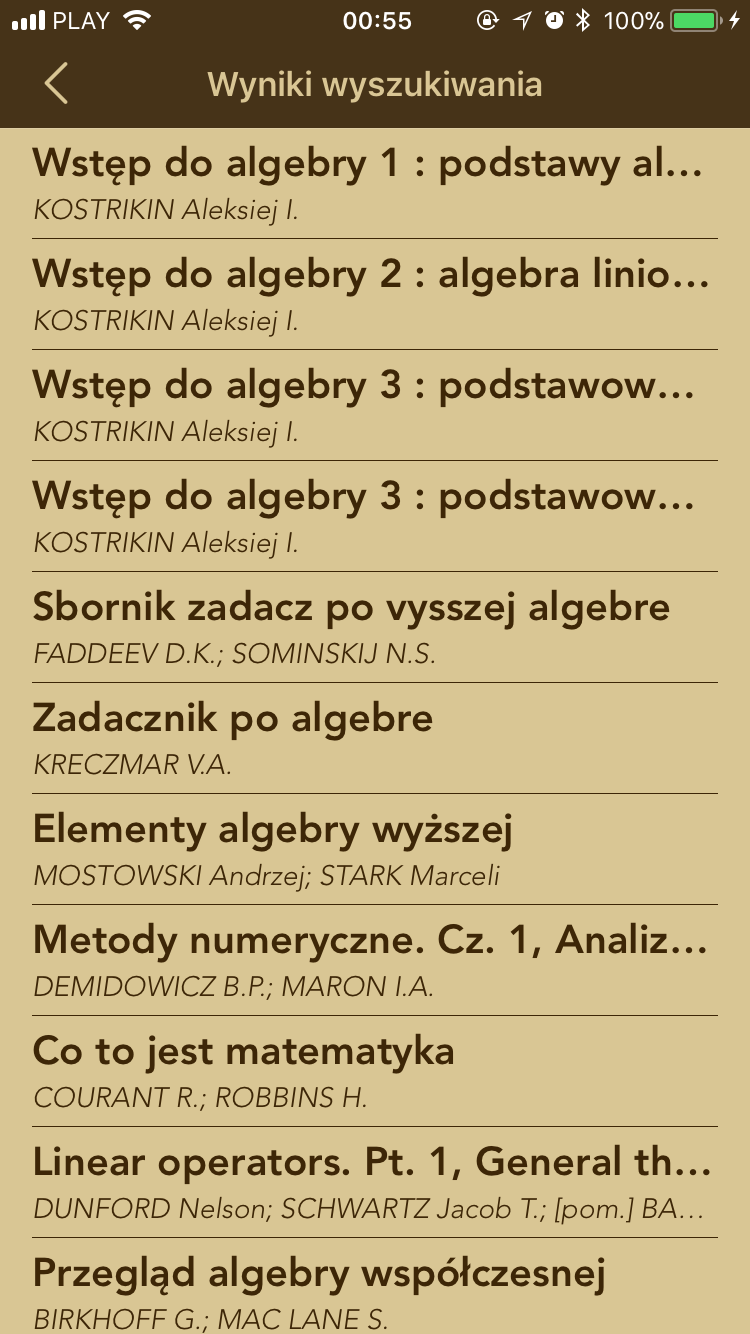
\includegraphics[width=0.8\linewidth]{img/iOS/ios4.PNG}
    \caption{Ekran wyników wyszukiwania}
    \label{fig:iosResults}
\end{minipage}%
\begin{minipage}{.5\textwidth}
    \centering
    
\includegraphics[width=0.8\linewidth]{img/iOS/ios5.PNG}
    \caption{Pusty ekran wyników}
    \label{fig:iosResultsEmpty}
\end{minipage}
\end{figure}

Użytkownik w celu przejścia dalej ma do wyboru dwie akcje:
\begin{enumerate}
\item Mocniejsze dociśnięcie ekranu w miejscu interesującej go pozycji.
\item Wybór interesującego go wiersza.
\end{enumerate}

\begin{figure}[h]
  \centering
  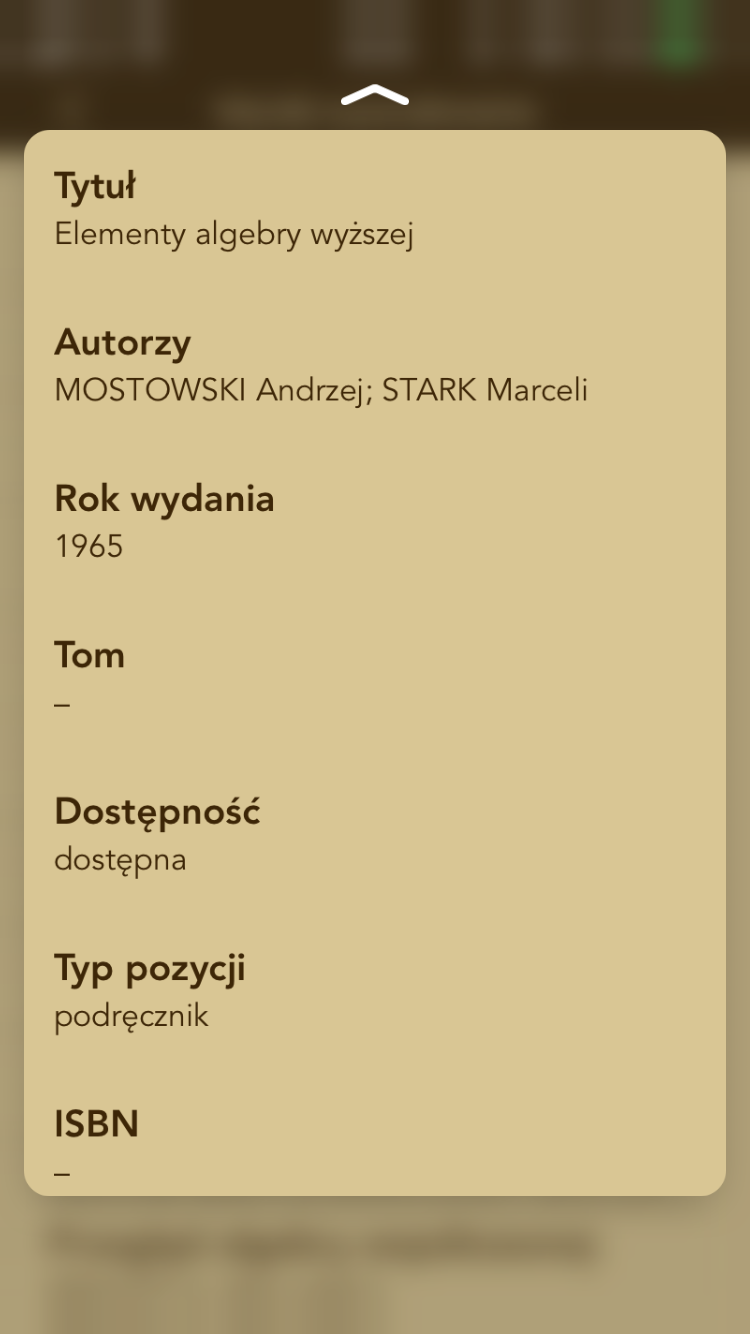
\includegraphics[width=0.4\linewidth]{img/iOS/ios6.PNG}
  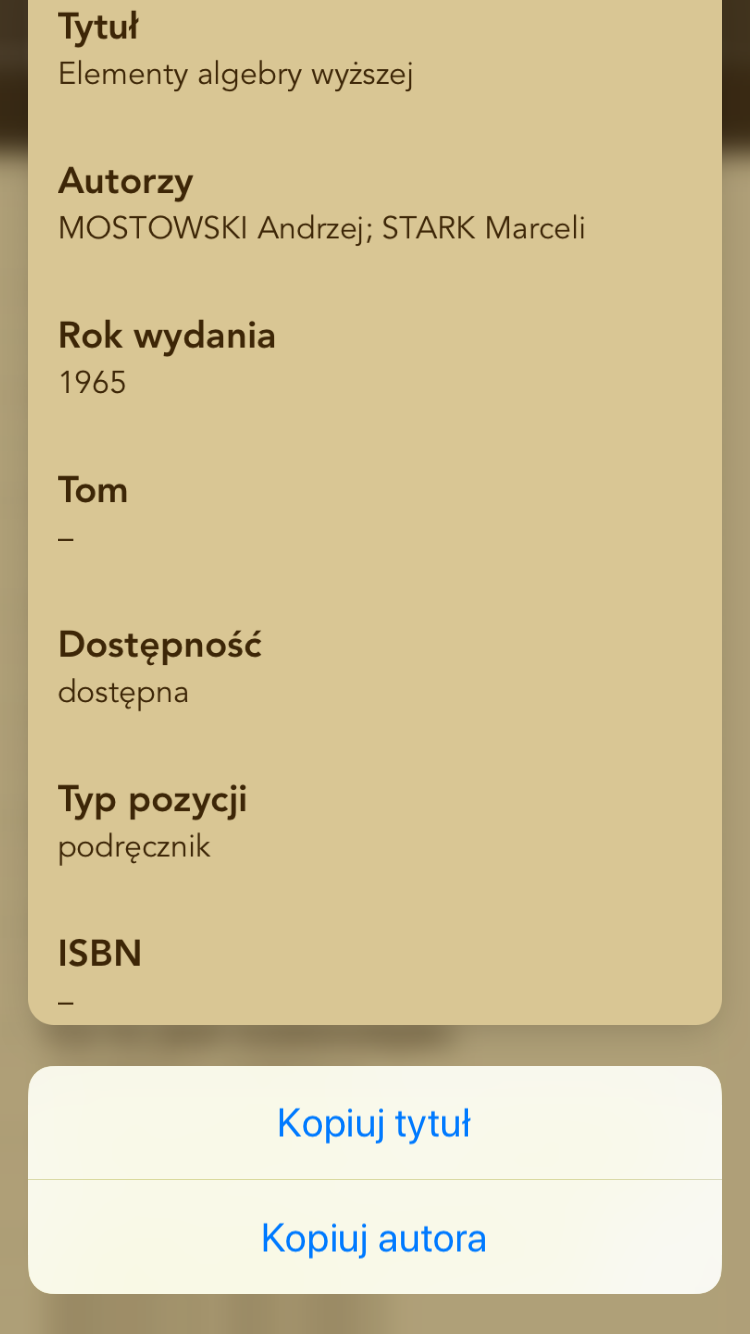
\includegraphics[width=0.4\linewidth]{img/iOS/ios7.PNG}
  \caption{Ekrany obsługujące akcje \textit{3D Touch}}
  \label{fig:3DTouch}
\end{figure}

Pierwsza opcja jest dostępna jedynie dla telefonów z opcją \textit{3D Touch} wbudowaną w ekran. W przypadku opcji 1., użytkownik otrzymuje na ekranie podgląd szczegółów książki, który przedstawiono na rysunku \ref{fig:3DTouch}. Przesunięcie go ku górze, spowoduje wyświetlenie się u dołu dodatkowych opcji. Będą to opcje umożliwiające skopiowanie tytułu bądź autora do schowka. Przeciągnięcie widoku podglądu w dół, spowoduje jego ukrycie. W przypadku jego jeszcze mocniejszego dociśnięcia, użytkownik zostanie przekierowany do ekranu. Analogiczna sytuacja ma miejsce podczas wyboru opcji numer 2., czyli zwykłego wyboru wiersza z książką.

W celu powrotu i rozpoczęcia szukania książki od początku, użytkownik może wybrać przycisk w lewym górnym rogu. Kliknięcie go, spowoduje powrót do ekranu wyszukiwania.

\subsubsection{Szczegóły książki}

Jest to ekran przedstawiony na rysunku \ref{fig:bookDetails}. Jest on prezentowany użytkownikowi od spodu, po wyborze jednej z komórek opisujących książkę. Przedstawia prostą przesuwaną listę elementów dotyczących wybranej książki. Przycisk w prawej górnej części ekranu pozwala schować widok i wrócić do poprzedniego ekranu wszystkich wyszukanych pozycji.

\begin{figure}[h]
  \centering
  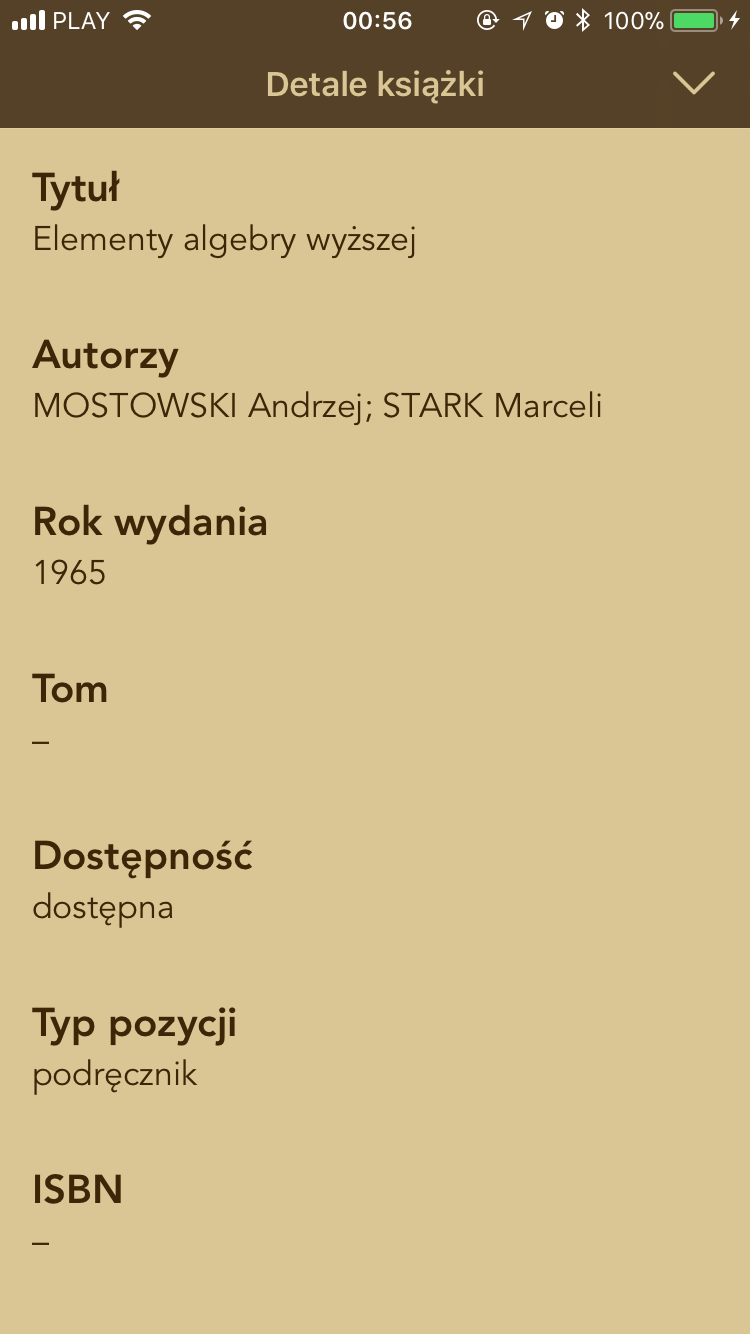
\includegraphics[width=0.4\linewidth]{img/iOS/ios8.PNG}
  \caption{Szczegóły książki}
  \label{fig:bookDetails}
\end{figure}


\section{Zakończenie}

Tworząc aplikację serwerową w tak małej grupie dla całego wydziału, mogliśmy znacznie poszerzyć swoją wiedzę o programowaniu, ale zarazem rozwinąć się w~zakresie pracy w zespole. Dodatkowo w celu lepszego porozumienia się z wieloma osobami, z którymi pracowaliśmy i dyskutowaliśmy podczas wytwarzania tej aplikacji, musieliśmy poszerzyć swoje zdolności interpersonalne. Bez ich pomocy byłoby nam ciężko dopracować wiele spraw związanych z dostosowaniem obsługi, a także wyglądu aplikacji dla klienta.

Cały projekt aplikacji mobilnych jak i aplikacji webowej został omówiony i wielokrotnie prezentowany oraz testowany z Panią mgr inż. Martyną Maciaszczyk, która była osobą zatwierdzającą wszystkie postanowienia oraz zmiany w widoku wszystkich aplikacji. Proces ten przebiegał stosunkowo długo, jednak był bardzo pouczający.

To właśnie interfejs graficzny był jednym z problemów wytworzenia takiego systemu. Bardzo trudne jest dostosowanie do siebie wszystkich aplikacji pod względem wyglądu. Strona internetowa zawsze będzie nieco inna od aplikacji mobilnej, ponieważ istnieje wiele różnic dotyczących założeń działania, obsługi, czy też przyzwyczajeń i wymagań użytkownika od danego systemu. Z tego powodu aplikacja internetowa dla administratora różni się od aplikacji mobilnych przeznaczonych przede wszystkim dla studentów. Największym problemem było dostosowanie do siebie obu aplikacji mobilnych na systemy Android i iOS. Każdą z nich pisała inna osoba, więc założenia dotyczące projektu musiały być dokładnie ustalone, a każda późniejsza edycja ponosiła za sobą modyfikacje na obu platformach, co przekładało się na dwukrotnie zwiększony czas potrzebny do realizacji danej zmiany. Dodatkowo każda z platform ma inne natywne narzędzia używane do tworzenia aplikacji. Systemy różnią się od siebie również wyglądem, co przyzwyczaja użytkowników do swoich rozwiązań. Z tego powodu aplikacje na dwa różne systemy nigdy nie mogą być identyczne jeśli chcą być intuicyjne dla ich grupy docelowej odbiorców.

Aplikacja serwerowa dla biblioteki została napisana w sposób łatwy do rozszerzenia. Jej wygodne i proste w obsłudze możliwości dodawania nowych książek do bazy, mogą być wykorzystywane w przyszłości w celu powiększania ilości zbiorów dostępnych w bibliotece. Dodatkowo, warto byłoby dodać możliwość rezerwacji książki online, bezpośrednio z poziomu aplikacji mobilnej. Ciekawą opcją na dalszą przyszłość (z powodu dużego nakładu pracy), byłaby możliwość wypożyczania danej pozycji książki w postaci pliku o rozszerzeniu .pdf. Pozwoliłoby to nie tylko na zmniejszenie kolejek w bibliotece, ale także na możliwość dostępu do wszystkich książek z~urządzenia przenośnego bez potrzeby noszenia dużej ich ilości przy sobie. Co więcej, ilość książek w tym wypadku byłaby nieograniczona. Każdy ze studentów miałby swój wirtualny egzemplarz. Niestety byłoby to możliwe do osiągnięcia jedynie przy dużym nakładzie pracy z powodu dużej ilości skanów do wykonania a także stworzenia nowej usługi pozwalającej na ściąganie i zapisywanie plików na urządzeniu przenośnym.

Celem naszego projektu było utworzenie systemu dla Biblioteki Wydziału Matematyki Stosowanej na Politechnice Śląskiej w Gliwicach. Cel ten udało nam się osiągnąć zgodnie ze wszystkimi założeniami jakie zostały przed nami postawione. Mamy nadzieję, że w przyszłości uda się wdrożyć nasz system do użytku, i że posłuży on gronu odbiorców w taki sposób, w jaki byśmy chcieli, aby służył nam, gdy faktycznie go potrzebowaliśmy.


\begin{thebibliography}{12}

\bibitem{raportBN} http://www.bn.org.pl/aktualnosci/1338-czytelnictwo-polakow-2016-\%E2\%80\%93-raport-biblioteki-narodowej.html [dostęp: 10 lutego 2018]
\bibitem{clean_code}
Robert C. Martin. 
\textit{Czysty kod. Podręcznik dobrego programisty}. 
Wydawnictwo Helion, 2010, ISBN 978-83-283-1401-6.
\bibitem{Swift1} The Swift Programming Language (Swift 4.0.3)
\bibitem{Swift2} Using Swift with Cocoa and Objective-C (Swift 4.0.3)
\bibitem{iosStatistics} https://developer.apple.com/support/app-store/ [dostęp: 10 lutego 2018]
\bibitem{AppleDeveloper} https://developer.apple.com/documentation/ [dostęp: 10 lutego 2018]
\bibitem{Rswift} https://github.com/mac-cain13/R.swift [dostęp: 10 lutego 2018]
\bibitem{JGProgressHUD} https://github.com/JonasGessner/JGProgressHUD
\bibitem{UIEmptyState} https://github.com/luispadron/UIEmptyState [dostęp: 10 lutego 2018]

\end{thebibliography}
\end{document}
